%% LyX 2.2.0 created this file.  For more info, see http://www.lyx.org/.
%% Do not edit unless you really know what you are doing.
\documentclass[english,notitlepage,showpacs,preprintnumbers,amsmath,amssymb,aps,nofootinbib,12pt]{revtex4-1}
\usepackage[T1]{fontenc}
\usepackage[latin9]{inputenc}
\setcounter{secnumdepth}{3}
\usepackage{color}
\usepackage{verbatim}
\usepackage{units}
\usepackage{amsmath}
\usepackage{amsthm}
\usepackage{amssymb}
\PassOptionsToPackage{normalem}{ulem}
\usepackage{ulem}

%pics 
\usepackage[pdftex]{graphicx}

%defs 
\newtheorem{theorem}{Theorem}[section]

\makeatletter
%%%%%%%%%%%%%%%%%%%%%%%%%%%%%% User specified LaTeX commands.
\usepackage{microtype}
\usepackage{xspace}
\usepackage{amsfonts}
\usepackage{palatino}
\usepackage[]{algorithm2e}
\usepackage{MnSymbol}
\usepackage{bbm}
%\usepackage{hyperref}
%\usepackage[hyphenbreaks]{breakurl1}
\usepackage{url}
\usepackage{ragged2e}
\edef\UrlBreaks{\do\-\UrlBreaks}% after loading url or hyperref
\usepackage{accents} % needed for \underbar that's same as \bar (\underaccent)
\usepackage{microtype}

\usepackage{color}

\newcommand*{\mathcolor}{}
\def\mathcolor#1#{\mathcoloraux{#1}}
\newcommand*{\mathcoloraux}[3]{%
  \protect\leavevmode
  \begingroup
    \color#1{#2}#3%
  \endgroup
}
%%% adding some commands to comment 
\usepackage{color}
%Some shortcuts added for edits
%Some shortcuts added for edits
% \usepackage{ulem}
\definecolor{dred}{rgb}{.8,0.2,.2}
\definecolor{ddred}{rgb}{.8,0.5,.5}
\definecolor{dblue}{rgb}{.2,0.2,.8}
% suggested change
\newcommand{\add}[1]{\textcolor{dred}{*#1*}} 
% \usepackage{ulem}
\newcommand{\out}[1]{\textcolor{ddred}{\textbf{[}#1\textbf{]}}}
% comment or remark
%\newcommand{\yo}[1]{\textcolor{dblue}{\textbf{[}#1\textbf{]}}}
% \newcommand{\todo}[1]{\textbf{\underline{\textcolor{dblue}{\textbf{[}#1\textbf{]}}}}}
%\newcommand{\jb}[1]{\textcolor{dblue}{\textbf{[}JB: #1\textbf{]}}}

\newcommand{\yo}[1]{\todo{{\textbf{[}JB: #1\textbf{]}}}}
\newcommand{\jb}[1]{\todo[inline]{{\textbf{[}JB: #1\textbf{]}}}}
%%%%%%%%%%



%% Set space of itemize environment
\usepackage{enumitem} % Used for setting height of itemize environments
\setlist[itemize]{topsep=0pt}%topsep=0pt


% Bookmarks in PDF (navigation pane)
\usepackage[colorlinks=true,linkcolor=black,urlcolor=black,bookmarksopen=true]{hyperref}
\usepackage{bookmark}

\newcommand{\hi}{$H_{\rm init}$\xspace}
\newcommand{\hf}{$H_{\rm final}$\xspace}

%% Set formatting of headers
\newcommand{\secspace}{\vspace{2mm}}

\newcommand{\summarysec}{\secspace\emph{\textbf{Summary}}}
\newcommand{\prossec}{\secspace\emph{\textbf{Pros}}}
\newcommand{\conssec}{\secspace\emph{\textbf{Cons}}}
\newcommand{\costsec}{\secspace\emph{\textbf{Cost}}}
\newcommand{\examplesec}{\secspace\emph{\textbf{Example}}}
\newcommand{\refsec}{\secspace\emph{\textbf{Bibliography}}}

\renewcommand{\baselinestretch}{1} % Single line spacing

\makeatother

\usepackage{babel}
\begin{document}

\vspace{-20mm}

\title{Quadratization in Pseudo-Boolean Optimization and Adiabatic Quantum
Computing}

\author{Richard Tanburn$^{1,\,}$}
%\email{richard.tanburn@hertford.ox.ac.uk}


\affiliation{$^{1}$Oxford University, Mathematical Institute, OX2 6GG, Oxford,
UK. }

\author{Nicholas Chancellor$^{2}$}
%\email{nicholas.chancellor@gmail.com}
\affiliation{$^{2}$Department of Physics, Durham University, DH1 3LE, South Road, Durham, UK.}

\author{Nikesh S. Dattani$^{3,4,5}$}
%\email{dattani.nike@gmail.com}
\affiliation{$^{3}$Harvard-Smithsonian Center for Astrophysics,}
\affiliation{$^{4}$McMaster University,}
\affiliation{$^{5}$Hertford College, Oxford University.}


\begin{abstract}
A collaborative, evolving, open review paper on $k$-local to 2-local transformations (quadratizations) in classical computing, quantum annealing, and universal adiabatic quantum computing.  
\end{abstract}

\maketitle


\title{\tableofcontents{}}

%\section{Introduction}
%
%%JB: I like the idea of entering with the general Ising model and then putting the quantum stuff a bit later on, otherwise it can confuse readers from the pseudoboolean background I fear. 
%
%\textbf{\emph{Every}} computation can be done by minimizing a Hamiltonian
%of either one of the following forms:
%
%\begin{eqnarray}
%H = \sum_{i}^{n} \left( \alpha_{i}z_{i}+\beta_{i}x_{i} \right) + \sum_{ij}^{n} \left( \alpha_{ij} z_{i}z_{j}+\beta_{ij}x_{i}x_{j} \right), \label{eq:XX+Z} \\
%H = \sum_{i}^{n} \left( \alpha_{i}z_{i}+\beta_{i}x_{i} \right) + \sum_{ij}^{n} \left( \alpha_{ij} z_{i}z_{j}+\beta_{ij}x_{i}z_{j} \right), \label{eq:XZ+Z}
%\end{eqnarray}
%where the $z$ and $x$ variables denote the Pauli matrices:
%\begin{equation}
%z\equiv\begin{pmatrix}1 & 0\\
%0 & -1
%\end{pmatrix},\,x\equiv\begin{pmatrix}0 & 1\\
%1 & 0
%\end{pmatrix},
%\end{equation}
%the $\alpha$ and $\beta$ coefficients are real numbers; and the Appendix will teach any unfamiliar readers how to interpret this notation.
%
%We know that every computation can be done this way because the minimization can be done by adiabatic quantum computation (AQC), and it has been proven \cite{Aharonov2008,Biamonte2008} that AQC can simulate any circuit-based quantum computation with overhead that grows at most polynomially with the size of the problem, and we know that circuit-based quantum computation can simulate any classical computation with at most polynomial overhead. %% Incorrect citation:  %Mizel2007
%If we remove all the terms in Eq. \ref{eq:XX+Z} or Eq. \ref{eq:XZ+Z} that have $x$ operators, we get an Ising Hamiltonian that is quadratic:
%\begin{equation}
%H=\sum_{i}^{n}\alpha_{i}z_{i}+\sum_{ij}^{n}\alpha_{ij}z_{i}z_{j},\label{eq:ZZ+Z}
%\end{equation}
%and we no longer know of any proof that \textbf{\emph{any}} computation can be done by minimizing such a Hamiltonian with only polynomial overhead compared to circuit-based quantum computation or even classical computation, but plenty of very interesting problems can still be formulated as the minimization or approximate minimization of a quadratic Ising Hamiltonian, such as neural network training \cite{Altaisky2016}, computerized image denoising \cite{Ishikawa2009,Ishikawa2011,Ishikawa2014,Anthony2015}, integer factorization \cite{Dattani2014}, and Ramsey number determination \cite{Gaitan2012,Bian2013}, just to name a few.
%However unlike Eq. \ref{eq:XZ+Z}, plenty of devices that can minimize Ising Hamiltonians already exist, and with further restrictions on the $\alpha$ coefficients, D-Wave has made devices with $n=2000$, and this number has roughly doubled every 14 months since the first 1-qubit demonstration in 2003, a phenomenon analogous to Moore's law of classical computer growth, which has become known as Rose's Law.
%
%Furthermore,\textbf{\emph{ no classical computer has ever been able to minimize certain quadratic Ising Hamiltonians faster than the D-Wave machines to date}} \cite{Denchev2016,Mandra2016}, so being able to turn computations into the form of Eq. \ref{eq:ZZ+Z} appears to be promising in terms of demonstrating the first useful application of quantum supremacy (which is the term used for quantum devices outperforming classical computation devices).
%Moreover, for problems like neural networks and computerized image denoising, the best known classical computation algorithms also work by turning the problems into minimizations of Ising Hamiltonians, so even if you are happy with continuing to only use classical computer and have no interest in using quantum annealing devices, turning a problem into a quadratic Ising Hamiltonian minimization problem can be very powerful for some computations.
%
%For neural networks, image denoising, integer factorization, and Ramsey number determination, it is rather easy to turn the problem into the form:
%
%\begin{equation}
%H=\sum_{i}^{n}\alpha_{i}z_{i}+\sum_{ij}^{n}\alpha_{ij}z_{i}z_{j}+\sum_{ijk}^{n}\alpha_{ijk}z_{i}z_{j}z_{k}+\sum_{ijkl}^{n}\alpha_{ijkl}z_{i}z_{j}z_{k}z_{l}\ldots,\label{eq:Z+ZZ+ZZZ+ZZZZ...}
%\end{equation}
%but then \textbf{\emph{quadratizing}} Eq. \ref{eq:Z+ZZ+ZZZ+ZZZZ...} into the quadratic Ising form often requires the introduction of auxiliary variables, and since minimizing Eq. \ref{eq:Z+ZZ+ZZZ+ZZZZ...} often has cost $\mathcal{O}(2^{n})$, it is often extremely desirable to do the quadratization with \textbf{\emph{as few auxiliary variables as possible}}.
%Apart from quadratizing with minimum number of variables, it is also often desirable to reduce the number of non-zero $\alpha$ coefficients, to keep the non-zero $\alpha$ coefficients bounded or with specific values, to reduce the number of positive (non-submodular) $\alpha$ coefficients, to reduce the spectral ratio of the Hamiltonian (`maximum energy minus
%minimum energy' divided by `energy of the second minimum minus the energy of the global minimum'), and to reduce the number of energy levels close to the global minimum.
%Adjusting the energy landscape in order to accomplish all of these things apart from reducing the number of auxiliary variables needed has been termed Energy Landscape Manipulation (ELM) which is an entirely separate topic, sometimes even more important than quadratizing with as few auxiliary variables as possible, nonetheless this Review simply focuses on methods for the latter aim.
%
%It has been shown in \cite{Anthony2015} that a general function of the form Eq. \ref{eq:Z+ZZ+ZZZ+ZZZZ...} with degree $k$, can be quadratized using $O(n^{k/2})$ auxiliary variables.
%However, it is often possible to quadratize with far fewer auxiliary variables (for example when the auxiliary variables for quadratizing one term are reused to quadratize other terms that have some of the same variables in them) or to quadratize without any auxiliaries at all (ex. if a Groebner basis can be found with all basis functions being quadratic, or if some symmetries in the Hamiltonian can be found that make it possible to quadratize without auxiliaries).
%
%\begin{comment}
%Also shown in \cite{Ishikawa2011} that a PSB in $n$ variables requires at most $2^{n}-1$ auxiliary variables (by representing it as a function of degree $n$).
%
%Positive quadratic terms (non-submodular), particularly with large positive coefficients, are hard for a lot of reasons, classically (Ishikawa TGBMM....) \cite{Ishikawa2011}.
%\end{comment}

\newpage

\part{{\normalsize{\underline{Diagonal Hamiltonians (pseudo-Boolean functions)}}}}

\section{Methods that introduce ZERO auxiliary variables}

\subsection{Deduction Reduction (Deduc-reduc)} \label{subsec:deduc_reduc}

\summarysec

We look for \emph{deductions} (e.g. $b_{1}b_{2}=0$) that hold at the global minimum.
These can be found by \emph{a priori} knowledge of the given problem, or by enumerating solutions of a small subset of the variables.
We can then substitute high-order terms using the low-order terms of the deduction, and add on a penalty term to preserve the ground states \cite{Tanburn2015c}.

\costsec
\begin{itemize}
\item $0$ auxiliary variables needed.%  Given a deduction, the reduction time is proportional to the number of terms in the Hamiltonian and is negligible. (but this is true of all the other reducs too)
\item The computational cost of the search for deductions is difficult to estimate.
The approximate worst-case complexity is $\mathcal{O}(n^{d+1}2^{m})$ where $m$ is the number of variables in a 'small' problem, $n$ is the total number of qubits and $d$ is the maximum degree of deductions we are searching for.
We suggest $10 \le m \le 20$, so that a small problem involves checking roughly $1,000$ to $1,000,000$ states, and $d=2$.
See the appendix for more details.
\end{itemize}

\prossec
\begin{itemize}
\item No auxiliary variables needed.
%\item Able to use extra information about a given problem.
\end{itemize}

\conssec
\begin{itemize}
\item When deductions cannot be determined naturally (as in the Ramsey number determination problem, see Example \ref{subsec:Example_Ramsey_deduc_reduc}), deductions need to be found by `brute force', which scales exponentially with respect to $m$.
For highly connected systems (systems with a large number of non-zero $\alpha_{ij}$ coefficients), the value of $m$ required to find even one deduction can be prohibitively large.
%\item Deductions do not always exist, or are too hard to find.
\end{itemize}

\examplesec

\begin{comment}
Examples are difficult to illustrate in a paper, since they involve searching for patterns in exhaustive searches. 
\end{comment}
Consider the Hamiltonian: 
\begin{equation}
H_{4{\rm -local}}=b_{1}b_{2}(10+b_{3}+b_{3}b_{4})+b_{1}(b_{3}-3)+b_{2}(b_{3}-2b_{3}-b_{4}-1)+F(x_{3},x_{4},x_{5},\ldots,x_{N})
\end{equation}
 where $F$ is any polynomial in $b_{i}$ for $i\ge 3$.

\noindent Since the $10$ coefficient of $b_{1}b_{2}$ is greater than the sum of all of the other coefficients involving $b_{1}$ or $b_{2}$, it must be the case that $b_{1}b_{2}=0$.
Specifically, for the 4 assignments of $(b_{3},b_{4})$, we see that $b_{1}b_{2}=0$ at every minimum of $H_{4{\rm -local}}-F$.

Using deduc-reduc we have:
\begin{equation}
H_{2{\rm -local}}=12b_{1}b_{2}+b_{1}(b_{3}-3)+b_{2}(b_{3}-2b_{3}-b_{4}-1)+F(x_{3},x_{4},x_{5},\ldots,x_{N})
\end{equation}

\noindent which has the same global minima as $H_{4-\textrm{local}}$ but one fewer quartic and one fewer cubic term.

\refsec
\begin{itemize}
\item Original paper, with application to integer factorization: \cite{Tanburn2015c}.
\end{itemize}

\newpage

\subsection{ELC Reduction}

\summarysec

An Excludable Local Configuration (ELC) is a partial assignment of variables that make it impossible to achieve the minimum.
We can therefore add a term that corresponds to the energy of this ELC without changing the solution to the minimization problem.
In practice we can eliminate all monomials with a variable in which a variable is set to 0, and reduce any variable set to 1.
Given a general Hamiltonian we can try to find ELCs by enumerating solutions of a small subset of variables in the problem \cite{Ishikawa2014}. 

\costsec
\begin{itemize}
\item $0$ auxiliary variables needed.
\item For $n$ qubits there is $\binom{n}{m}$ ways to choose $m$ of them and $2^m$ assignments of these $m$ variables, therefore $\mathcal{O}\left(2^{m}\binom{n}{m}\right)$ operations required to enumerate all possible cases for all possible subsets of size $m \le n$ variables.
\item Approximate methods exist which have been shown to be much faster and give good approximations to the global minimum \cite{Ishikawa2014}.
\end{itemize}

\prossec
\begin{itemize}
\item No auxiliary variables needed.
\end{itemize}

\conssec
\begin{itemize}
\item No known way to find ELCs except by `brute force', which scales exponentially with respect to $m$. 
\item ELCs do not always exist.
\end{itemize}

\examplesec

Consider the Hamiltonian: 
\begin{equation}
H_{{\rm 3-local}}=b_{1}b_{2}+b_{2}b_{3}+b_{3}b_{4}-4b_{1}b_{2}b_{3}. \label{eq:ELCexample}
\end{equation}
If $b_{1}b_{2}b_{3}=0$, no assignment of our variables will we be able to reach a lower energy than if $b_{1}b_{2}b_{3}=1$.
Hence this gives us 12 ELCs, and one example is $(b_{1},b_{2},b_{3})=(1,0,0)$ which we can use to form the polynomial:
\begin{align}
H_{2\rm{-local}}&=H_{{\rm 3-local}}+4b_{1}(1-b_{2})(1-b_{3})\\
&=b_{1}b_{2}+b_{2}b_{3}+b_{3}b_{4}+4b_{1}-4b_{1}b_{2}-4b_{1}b_{3}. \label{eq:ELCreduced}
\end{align}
In both cases Eqs. \eqref{eq:ELCexample} and \eqref{eq:ELCreduced}, the only global minima occur when $b_1b_2b_3 = 1$.

\refsec
\begin{itemize}
\item Original paper and application to computerized image denoising: \cite{Ishikawa2014}.
\end{itemize}



\newpage
\subsection{Groebner Bases}

\begin{comment}
% Nike's old summary
A Groebner basis is a set of equations representing the zeros of a polynomial (e.g. of the form Eq. \ref{eq:Z+ZZ+ZZZ+ZZZZ...}) such that the number of variables is the same, and the zeros of Eq. \ref{eq:Z+ZZ+ZZZ+ZZZZ...} are the same as the zeros of all equations of the Groebner basis.
If a Groebner basis can be found such that all equations are quadratic, then quadratization of Eq. \ref{eq:Z+ZZ+ZZZ+ZZZZ...} is as simple as finding the Groebner basis.

\begin{comment}
Nike, this is NOT true.
Once we have the Groebner basis, we still need a single non-negative expression to minimize.
This involves finding appropriate coefficients of the equations to add together (non-trivial and what they do in the 1Qbit paper) OR squaring each one, which gives a quartic. 
\end{comment}

\begin{comment}
Use the multivariate extension of Gaussian elimination to find a different set of equations which have the same vanishing set.
It has been shown these can be used to reduce and embed factorisations of all bi-primes up to 200,000 \cite{Dridi2016}.
Some work has been done in the field of ``boolean Groebner bases'', but these consider bases of a boolean ring over $\mathbb{F}_{2}$ rather than $\mathbb{Q}$.
\end{comment}

%% Old description
\begin{comment}
\textcolor{red}{Richard: too much algebra here. People come from different
backgrounds. Some people don't know what rings are, and some people
get scared when they see fancy symbols like $\mathcal{V}$. It should
be possible to describe this to A-level students because that way
we know everyone (chemists, physicists, engineers, computer scientsists,
etc.) will understand it. I guess I already did this in a way that
A-level students would understand, in the ``summary section''. For
``descriptions'' I envision that we explain exactly how to DO the
methods, and for Groebner bases, I guess this would be equivalent
to listing the known algorithms (such as Buchberger's) and known codes
available. I guess another description that could be added is the
method in the 1Qbit paper, where they have a ``max\_cutoff'' and
a ``min\_cutoff'' and Groebnerized everything in between there,
or something like that.}

Instead of solving the equations $f_{1}=f_{2}=...=f_{n}=0$ directly,
Groebner bases consider the points on which they vanish, also known
as the \emph{algebraic variety} $\mathcal{V}(f_{1},...,f_{n})$. Groebner
bases are a 'pleasant' generating set for this variety.

This is done by first defining a monomial ordering on the polynomial
ring $F[b_{1},...,b_{n}]$, chosen so that higher order mononials
are considered 'bigger' than low order monomials. Monomials of the
same degree are sorted by the lexicographic ordering of the variables.
Then define the leading term of a polynomial $f$ with respect to
the monomial ordering to be $\mathrm{LT}(f)$, the largest monomial
of $f$. Then $g_{1},...,g_{m}$ is a Grobner basis if $\mathcal{V}(f_{1},...,f_{n})$=$\mathcal{V}(g_{1},...,g_{m})$
(they have the same vanishing set) and for every function $f$ in
the ideal of $\left\langle f_{1},...f_{n}\right\rangle $, we have
that the leading term of $f$ is divisible by the leading term of
$g_{i}$ for some $i$.

Grobner bases are very useful because they allow computation of remainders,
using the multivariate division algorithm. They are useful in this
context since the polynomials of the Grobner basis will have smaller
degrees than our original function, reducing the need for reduction
by other means.
\end{comment}

\summarysec

Given a set of polynomials, a Groebner basis is another set of polynomials that have exactly the same zeros.
The advantage of a Groebner basis is it has nicer algebraic properties than the original equations, in particular they tend to have smaller degree polynomials.
The algorithms for calculating Groebner bases are generalizations of Euclid's algorithm for the polynomial greatest common divisor.

Work has been done in the field of 'Boolean Groebner bases', but while the variables are Boolean the coefficients of the functions are in $\mathbb{F}_{2}$ rather than $\mathbb{Q}$.

\costsec
\begin{itemize}
\item $0$ auxiliary variables needed.
\item $\mathcal{O}\left( 2^{2^{n}} \right)$ in general, $\mathcal{O}(d^{n^{2}})$ if the zeros of the equations form a set of discrete points, where $d$ is the degree of the polynomial and $n$ is the number of variables \cite{Bardet2002}.
\end{itemize}

\prossec
\begin{itemize}
\item No auxiliary variables needed.
\item General method, which can be used for other rings, fields or types of variables.
\end{itemize}

\conssec
\begin{itemize}
\item Best algorithms for finding Groebner bases scale double exponentially in $n$.
\item Only works for Hamiltonians whose minimization corresponds to solving systems of discrete equations (RICHARD, why is this the ONLY case?).
\end{itemize}

\examplesec

Consider the following pair of equations:

\begin{equation}
b_1 b_2 b_3 b_4 + b_1 b_3 + b_2 b_4 - b_3 = b_1 + b_1 b_2 + b_3 - 2 = 0.
\end{equation}

\noindent Feeding these to Mathematica's ${\tt GroebnerBasis}$ function, along with the binarizing $b_1(b_1-1)=\ldots=b_4(b_4-1)=0$ constraints, gives a Groebner basis:

\begin{equation}
\left\{ b_4 b_3 - b_4, b_2 + b_3 - 1, b_1 - 1 \right\}.
\end{equation}

From this we can immediately read off the solutions $b_1=1$, $b_2=1-b_3$ and reduce the problem to $b_3b_4-b_4=0$. Solving this gives a final solution set of: $(b_1, b_2, b_3, b_4) = (1, 0, 1, 0), (1, 0, 1, 1), (1, 1, 0, 0)$.

\refsec
\begin{itemize}
%\item Standard text on Computational Algebraic Geometry: \cite{Cox2007}.
\item Reduction and embedding of factorizations of all bi-primes up to $200,000$: \cite{Dridi2016}.
\end{itemize}

\begin{comment}
To quadratize the Hamiltonian: 
\begin{equation}
H_{4{\rm -local}}=(z_{1}z_{2}-z_{3}z_{4}-1)^{2},
\end{equation}
we first linearize the part that is being squared. In Mathematica,
the ${\tt GroebnerBasis}$ function gives us:

Then when we square it we get a quadratic function:

\begin{equation}
H_{2{\rm -local}}=1-2z_{1}-2z_{2}+3z_{3}+3z_{4}-2z_{3}z_{4}.
\end{equation}
In both cases, the only global minima occur when:

\begin{equation}
(z_{3,}z_{4})=1,\,z_{1}\,\text{or}\,z_{2}=0.
\end{equation}

\textcolor{red}{Wait, this is far from true!}
\end{comment}
\newpage

\subsection{Split Reduction}

\summarysec

It has been shown in \cite{Okada2015} that, if multiple runs of a minimization algorithm is permitted, it is possible to reduce a lot of the problem by conditioning on the most connected variables.
We call each of these operations a \emph{split}.

\costsec

Exponential in the number of splits, as the number of problems to solve doubles with every split.

\prossec
\begin{itemize}
\item This method can be applied to any problem and can be very effective on problems with a few very connected variables.
\end{itemize}

\conssec
\begin{itemize}
\item Exponential cost in the worst case.
\end{itemize}

\examplesec

Consider the simple objective function 
\begin{equation}
H=1+b_{1}b_{2}b_{5}+b_{1}b_{6}b_{7}b_{8}+b_{3}b_{4}b_{8}-b_{1}b_{3}b_{4}.
\end{equation}
In order to quadratize $H$, we first have to choose a variable to split over.
In this case $b_{1}$ is the obvious choice since it is present in the most terms and contributes to the quartic term.

We then obtain two different problems:
\begin{eqnarray}
H_{0} & = & 1+b_{3}b_{4}b_{8}\\
H_{1} & = & 1+b_{2}b_{5}+b_{6}b_{7}b_{8}+b_{3}b_{4}b_{8}-b_{3}b_{4}.
\end{eqnarray}

At this point, we could split $H_{0}$ again and solve it entirely, or use a qubit we saved in the previous split to quadratize our only problem.

To solve $H_{1}$, we can split again on $b_{8}$, resulting in problems:
\begin{eqnarray}
H_{1,0} & = & 1+b_{2}b_{5}+b_{6}b_{7}\\
H_{1,1} & = & 1+b_{2}b_{5}+b_{3}b_{4}.
\end{eqnarray}
Now both of these problems are quadratic.
Hence we have reduced our original, hard problem into 3 easy problems, requiring only 2 extra runs of our minimization algorithm, and without needing any auxiliary variables.

\refsec
\begin{itemize}
\item Original paper and application to Ramsey number calculation: \cite{Okada2015}.
\end{itemize}

\newpage
\section{Methods that introduce auxiliary variables to quadratize a SINGLE term}

\subsection{Negative Term Reduction} \label{subsec:Negative-Monomial-Reduction}

\summarysec

For a negative term $-b_{1}b_{2}...b_{k}$, introduce a single auxiliary variable $b_a$ and make the substitution:
\begin{equation}
-b_{1}b_{2} \ldots b_{k} = \min_{b_a} \left( (k-1-\sum_i b_{i})b_a \right).
\end{equation}

\costsec
\begin{itemize}
\item 1 auxiliary variable for each $k$-local term.
\end{itemize}

\prossec
\begin{itemize}
\item All resulting quadratic terms are submodular (have negative coefficients).
\item Can reduce arbitrary order terms with only 1 auxiliary.
%\item Can be generalized so that one variable can be made to work for multiple terms.% (I can't find anyone saying this, but can be proven. Look at the commented out example below!)
\end{itemize}

\conssec
\begin{itemize}
\item Only works for negative terms.
\end{itemize}

\examplesec

\begin{align}
H_{{\rm 6-local}} & =-2b_{1}b_{2}b_{3}b_{4}b_{5}b_{6} + b_5b_6,
\end{align}
has a unique minimum energy of -1 when all $b_i=1$.

\begin{equation}
H_{{\rm 2-local}}=2\left( 5b_a-b_{1}b_a-b_{2}b_a-b_{3}b_a-b_{4}b_a-b_{5}b_a-b_{6}b_a \right) + b_5b_6
\end{equation}
has the same unique minimum energy, and it occurs at the same place (all $b_i=1$), with $b_a=1$.

\begin{comment}
\examplesec
\begin{align}
H_{{\rm 5-local}} & =-b_{1}b_{2}b_{3}b_{4}b_{5}-b_{1}b_{2}b_{3}b_{4}b_{6},
\end{align}
has a unique minimum energy of -2 when all $b$'s are 1.

\begin{equation}
H_{{\rm 3-local}}=(3-b_{1}-b_{2}-b_{3}-b_{4})(b_{5}+b_{6})a
\end{equation}
has the same unique minimum energy, and it occurs at the same place,
with $a=1$.
\end{comment}

\refsec
\begin{itemize}
\item Original paper: \cite{Freedman2005}.
\item Discussion: \cite{Ishikawa2011}, \cite{Anthony2015}.
\end{itemize}

\newpage

\subsection{Positive Term Reduction}

\summarysec

By considering the negated literals $\bar{b}_{i}=1-b_{i}$, we recursively apply the previous method to $b_{1}b_{2}\ldots b_{k}=-\bar{b}_{1}b_{2}\ldots b_{k}+b_{2}b_{3}\ldots b_{k}$.
The final identity is:
\begin{equation}
b_{1}b_{2}\ldots b_{k}=\min_{b_a}\left(\sum_{i=1}^{k-2}b_{a_{i}}(k-i-1+b_{i}-\sum_{j=i+1}^{k}b_{j})\right)+b_{k-1}b_{k}
\end{equation}


\costsec
\begin{itemize}
\item $k-2$ auxiliary variables for each $k$-local term.
\end{itemize}

\prossec
\begin{itemize}
\item Works for positive monomials.
\end{itemize}

\conssec
\begin{itemize}
\item $k-1$ non-submodular quadratic terms.
\end{itemize}

\examplesec
\begin{eqnarray}
b_{1}b_{2}b_{3}b_{4} & = & \min_{b_a}{b_{a_{1}}(2+b_{1}-b_{2}-b_{3}-b_{4})+b_{a_{2}}(1+b_{2}-b_{3}-b_{4})}+b_{3}b_{4}
\end{eqnarray}

\refsec
\begin{itemize}
\item Summary: \cite{Boros2014}.
\end{itemize}

\begin{comment}
By flipping and applying \ref{subsec:Negative-Monomial-Reduction} alternatively, we get a nice way to reduce a quartic using only 2 variables and with only 2 positive terms and much less connectivity:

\begin{eqnarray}
b_{1}b_{2}b_{3}b_{4} & \mapsto & b_{2}b_{3}b_{4}-\bar{b}_{1}b_{2}b_{3}b_{4}\\
 & \mapsto & b_{2}b_{3}b_{4}+\big(3a_{1}-a_{1}(\bar{b}_{1}+b_{2}+b_{3}+b_{4})\big)\\
 & \mapsto & b_{3}b_{4}-\bar{b}_{2}b_{3}b_{4}+\big(3a_{1}-a_{1}(\bar{b}_{1}+1-\bar{b}_{2}+b_{3}+b_{4})\big)\\
 & \mapsto & b_{3}b_{4}+\big(2a_{2}-a_{2}(\bar{b}_{2}+b_{3}+b_{4}\big)\big)+\big(3a_{1}-a_{1}(\bar{b}_{1}+1-\bar{b}_{2}+b_{3}+b_{4})\big)\\
 & \mapsto & b_{3}b_{4}+a_{2}+a_{2}b_{2}-a_{2}b_{3}-a_{2}b_{4}+2a_{1}+a_{1}b_{1}-a_{1}b_{2}-a_{1}b_{3}-a_{1}b_{4}
\end{eqnarray}
\end{comment}

\newpage

\subsection{Ishikawa's Symmetric Reduction (Positive Term Reduction)}

\summarysec

This method rewrites a positive monomial using symmetric polynomials, so all possible quadratic terms are produced and they are all non-submodular: 
\begin{equation}
b_{1}...b_{k} = \min_{b_{a_1}, \ldots, b_{a_{n_k}}} \left( \sum_{i=1}^{n_{k}}b_{a_{i}}\left(c_{i,d}\left(-\sum_{j=1}^{k}b_{j}+2i\right)-1\right)+\sum_{i<j}b_{i}b_{j} \right)
\end{equation}
where $n_{k}=\left\lfloor \frac{k-1}{2}\right\rfloor $ and $c_{i,k}=\begin{cases}
1, & i=n_{d}\text{ and }k\text{ is odd,}\\
2, & \text{else.}
\end{cases}$

\costsec
\begin{itemize}
\item $\left\lfloor \frac{k-1}{2}\right\rfloor $ auxiliary variables for each $k$-order term
\item $\mathcal{O}(kt)$ for a $k$-local Hamiltonian with $t$ terms.
\end{itemize}

\prossec
\begin{itemize}
\item Works for positive monomials.
About half as many auxiliary variables for each $k$-order term as the previous method.
\end{itemize}

\conssec
\begin{itemize}
\item $\mathcal{O}(k^{2})$ quadratic terms are created, which may make chimerization more costly.
\item $\frac{k(k-1)}{2}$ non-submodular terms.
\item Worse than the previous method for quartics, with respect to submodularity.
\end{itemize}

\examplesec
\begin{eqnarray}
b_{1}b_{2}b_{3}b_{4} & = & \min_{b_a}(3-2b_{1}-2b_{2}-2b_{3}-2b_{4})b_a+b_{1}b_{2}+b_{1}b_{3}+b_{1}b_{4}+b_{2}b_{3}+b_{2}b_{4}+b_{3}b_{4}
\end{eqnarray}

\refsec
\begin{itemize}
\item Original paper and application to image denoising: \cite{Ishikawa2011}.
\end{itemize}
\newpage

\subsection{Asymmetric Reduction}

\summarysec

Similar to other methods of reducing one term, this method can reduce a positive cubic monomial into quadratic terms using only one auxiliary variable, while introducing fewer non-submodular terms than the symmetric version.


The identity is given by:
\begin{align}
b_{1}b_{2}b_{3}&= \min_{b_a} \left( b_a-b_{2}b_a-b_{3}b_a+b_{1}b_a+b_{2}b_{3} \right)\\
               &= \min_{b_a} \left( b_a-b_{1}b_a-b_{3}b_a+b_{2}b_a+b_{1}b_{3} \right)\\
               &= \min_{b_a} \left( b_a-b_{1}b_a-b_{2}b_a+b_{3}b_a+b_{1}b_{2} \right)\\
\end{align}

\costsec

1 auxiliary qubit per positive cubic term.

\prossec
\begin{itemize}
\item Works on positive monomials.
\item Fewer non-submodular terms than Ishikawa Reduction.
\end{itemize}

\conssec
\begin{itemize}
\item Only been shown to work for cubics.
\end{itemize}

\refsec
\begin{itemize}
\item Original paper and application to computer vision: \cite{Gallagher2011}.
\end{itemize}

\newpage
\subsection{Bit flipping}

\summarysec

For any variable $b$, we can consider the negation $\bar{b}=1-b$.
The process of exchanging $b$ for $\bar{b}$ is called \emph{flipping}.
Using bit-flipping, an arbitrary function in $n$ variables can be represented using at most $2^{(n-2)}(n-3)+1$ variables, though this is a gross overestimate.

Can be used in many different ways:
\begin{enumerate}
\item Flipping positive terms and using \ref{subsec:Negative-Monomial-Reduction}, recursively;
\item For $\alpha<0$, we can reduce $\alpha\bar{b}_{1}\bar{b}_{2}...\bar{b}_{k}$ very efficiently to submodular form using \ref{subsec:Negative-Monomial-Reduction}.
A generalized version exists for arbitrary combinations of flips in the monomial which makes reduction entirely submodular \cite{Ishikawa2011};
\item When we have quadratized we can minimize the number of non-submodular terms by flipping.
\item We can make use of both $b_{i}$ and $\bar{b}_{i}$ in the same Hamiltonian by adding on a sufficiently large penalty term: $\lambda(b_{i}+\bar{b}_{i}-1)^{2}=\lambda(1+2b_{i}\bar{b}_{i}-b_{i}-\bar{b}_{i})$.
This is similar to the ideas in reduction by substitution or deduc-reduc.
In this way, given a quadratic in $n$ variables we can make sure it only has at most $n$ nonsubmodular terms if we are willing to use the extra $n$ negation variables as well (so we have $2n$ variables in total).
\end{enumerate}

\costsec
\begin{itemize}
\item None, as replacing $b_{i}$ with it's negation $\bar{b}_{i}$ costs nothing except a trivial symbolic expansion.
\end{itemize}

\prossec
\begin{itemize}
\item Cheap and effective way of improving submodularity.
\item Can be used to combine terms in clever ways, making other methods more efficient.
\end{itemize}

\conssec
\begin{itemize}
\item Unless the form of the Hamiltonian is known, spotting these 'factorizations' using negations is difficult.
\item We need an auxiliary variable for each $b_i$ for which we also want to use $\bar{b_i}$ in the same Hamiltonian.
\end{itemize}

\examplesec

By bit-flipping $b_2$ and $b_4$, i.e. substituting $b_2 = 1 - \bar{b}_{2}$ and $b_4 = 1 - \bar{b}_{4}$, we see that:
\begin{eqnarray}
H & = & 3b_{1}b_{2}+b_{2}b_{3}+2b_{1}b_{4}-4b_{2}b_{4}\protect\\
 & = & -3b_{1}\bar{b}_{2}-\bar{b}_{2}b_{3}-2b_{1}\bar{b}_{4}-\bar{b}_{2}\bar{b}_{4}+5b_{1}+b_{3}+4\bar{b}_{2}+4\bar{b}_{4}-4.
\end{eqnarray}
The first expression is highly non-submodular while the second is entirely submodular.

\refsec
\begin{itemize}
\item Original paper: \cite{Ishikawa2011}.
\end{itemize}

\section{Methods that introduce auxiliary variables to quadratize MULTIPLE terms with the SAME auxiliaries}

\subsection{Reduction by Substitution}

\summarysec

Pick a variable pair $(b_{i},b_{j})$ and substitute $b_{i}b_{j}$ with a  new auxiliary variable $b_{a_{i,j}}$.
Enforce equality in the ground states by adding some scalar multiple of $b_{i}b_{j}-2b_{i}b_{a_{i,j}}-2b_{i}b_{a_{i,j}}+3b_{a_{i,j}}$ or similar.

\costsec
\begin{itemize}
\item 1 auxiliary variable per reduction.
\end{itemize}

\prossec
\begin{itemize}
\item Variable can be used across the entire Hamiltonian, reducing many terms at once.
\item Simple.
\end{itemize}

\conssec
\begin{itemize}
\item Inefficient for single terms as it introduces many auxiliary variables compared to Ishikawa reduction, for example.
\item Introduces quadratic terms with large positive coefficients, making them highly non-submodular.
\item Determining optimal substitutions is expensive.
\end{itemize}

\examplesec

We pick the pair $(b_{1},b_{2})$ and combine.

\begin{equation}
b_{1}b_{2}b_{3}+b_{1}b_{2}b_{4}\mapsto b_{3}b_a+b_{4}b_a+b_{1}b_{2}-2b_{1}b_a-2b_{1}b_a+3b_a
\end{equation}

\refsec
\begin{itemize}
\item Original paper: \cite{Rosenberg1975}
\end{itemize}

\newpage
\subsection{FGBZ Reduction (Fix-Gruber-Boros-Zabih)}

\summarysec

Here we consider a set $C$ of variables which occur in multiple monomials throughout the Hamiltonian.
Each application 'rips out' this common component from each term \cite{Fix2011}\cite{Boros2014}.

Let $\mathcal{H}$ be a set of monomials, where $C \subseteq H$ for each $H\in\mathcal{H}$ and each monomial $H$ has a weight $\alpha_{H}$.
The algorithm comes in 2 parts: when all $\alpha_{H}>0$ and when all $\alpha_{H}<0$. Combining the 2 gives the final method:

\begin{enumerate}
\item $\alpha_{H}>0$ 
\begin{equation}
\sum_{H\in\mathcal{H}}\alpha_{H}\prod_{j\in H}b_{j}=\min_{b_a}\left(\sum_{H\in\mathcal{H}}\alpha_{H}\right)b_a\prod_{j\in C}b_{j}+\sum_{H\in\mathcal{H}}\alpha_{H}(1-b_a)\prod_{j\in H\setminus C}b_{j}
\end{equation}
\item $\alpha_{H}<0$
\begin{equation}
\sum_{H\in\mathcal{H}}\alpha_{H}\prod_{j\in H}b_{j}=\min_{b_a}\sum_{H\in\mathcal{H}}\alpha_{H}\left(1-\prod_{j\in C}b_{j}-\prod_{j\in H\setminus C}b_{j}\right)b_a
\end{equation}
\end{enumerate}

\costsec
\begin{itemize}

\item One auxiliary variable per application.
\item In combination with \ref{subsec:Negative-Monomial-Reduction}, it can be used to make an algorithm which can reduce $t$ positive monomials of degree $d$ in $n$ variables using $n+t(d-1)$ auxiliary variables in the worst case.
\end{itemize}

\prossec
\begin{itemize}
\item Can reduce the connectivity of a Hamiltonian, as it breaks interactions between variables.
\end{itemize}

\conssec
\begin{itemize}
\item $\alpha_{H}>0$ method converts positive terms into negative ones of same order rather than reducing them, though these can then be reduced more easily.
\item $\alpha_{H}<0$ method only works for $|C|>1$, and cannot quadratize cubic terms.
\end{itemize}

\examplesec

First let $C=b_{1}$ and use the positive weight version:
\begin{eqnarray}
b_{1}b_{2}b_{3}+b_{1}b_{2}b_{4} & \mapsto & 2b_{a_1}b_{1}+(1-b_{a_1})b_{2}b_{3}+(1-b_{a_1})b_{2}b_{4}\\
 & = & 2b_{a_1}b_{1}+b_{2}b_{3}+b_{2}b_{4}-b_{a_1}b_{2}b_{3}-b_{a_1}b_{2}b_{4}
\end{eqnarray}
now we can use \ref{subsec:Negative-Monomial-Reduction}:

\begin{eqnarray}
-b_{a_1}b_{2}b_{3}-b_{a_1}b_{2}b_{4} & \mapsto & 2b_{a_2}-b_{a_1}b_{a_2}-b_{a_2}b_{2}-b_{a_2}b_{3}+2b_{a_2}-b_{a_1}b_{a_2}-b_{a_2}b_{2}-b_{a_2}b_{4}\\
 & = & 4b_{a_2}-2b_{a_1}b_{a_2}-2b_{a_2}b_{2}-b_{a_2}b_{3}-b_{a_2}b_{4}.
\end{eqnarray}

\refsec
\begin{itemize}
\item Original paper and application to image denoising: \citep{Fix2011}.
\end{itemize}

\begin{comment}

\subsection{Generalized roof duality}

(only 1 extra qubit, but only works for up to 5-qubit terms.)

Nike, where did you get the above from? When I search for this, with
the relevant authors, I only find stuff on QPBO. I've spent a while
reading papers on QPBO (fascinating stuff, very impressive and in
some ways similar to what we've been trying/will try to do. Is the
quantum community aware of their software??). I don't know what roof
duality you're referring to.

\subsection{Generalized Roof Duality (QPBO)}

\summarysec

Algorithm that takes a quadratic Hamiltonian and tries to perform as much of the optimization as possible.

\costsec

For computer image problems, it can be used with the above methods to optimize most of the image in seconds/minutes \cite{Ishikawa2014,Fix2011,Ishikawa2011}.
\end{comment}


\section{Methods that reproduce the full spectrum}

%All known methods to map the entire spectrum of a Hamiltonian rely on the same basic principle: auxilliary variables are added, to mediate the high-order interactions, and constraints are added to restrict the values which the axilliary variables can take. In practice, constraints are implemented as one and two term equations with much stronger energy penalties than those in the original Hamiltonian. As long as the constraints are sufficiently strong, the low energy subspace of the 2-local Hamiltonian will be exactly the spectrum of the original $k$-local Hamiltonian. Moreover, the location of the original `logical' variables is known and so the resulting configuration of the mapped variables can easily be determined.

%If we want to reproduce the spectrum of  $b_1b_2b_3$, (such that the state $b_1=1,b_2=1,b_3=1$ will have energy $1$ and all others will have energy $0$)  we need to find a quadratic penalty function $P(a,b_1,b_2)$ such that if an auxilliary variable $a$ satisfies $a=b_1b_2$, $P(a,b_1,b_2)=0$, and $P(a,b_1,b_2)>0$ otherwise. If we can find such a function (we explain how to do this is subsection \ref{sub:recursive}), then the desired spectrum will be reproduced in the low energy sector of the following Hamiltonian.

%\begin{equation}
%H_{3-\rm{local}}=b_3\,a+\lambda\,P(a,b_1,b_2)
%\end{equation}

%\noindent where $\lambda$ is a large positive number.

These techniques will transform $k$-local functions to 2-local functions that not only have the same ground state as the $k$-local function, but also the entire input/output spectrum of the $k$-local functions will be preserved in the low-lying energy space of the corresponding 2-local function (which also has higher energy states due to the auxiliary variables added). 


\subsection{Recursive Order Reduction\label{sub:recursive}}

\summarysec

For each $k$-local term an auxilliary variable and a quadratic penalty function to constrain the auxilliary variable, is used to reduce the term's order to $(k-1)$-local. This is repeated recursively until the term is 2-local.

\costsec
\begin{itemize}
\item $k-2$ auxiliary variables to reduce each $k$-local terms.
\item  At most $k\,t$ for a $k$-local Hamiltonian of $t$ terms.
\end{itemize}

\prossec
\begin{itemize}
\item  Simple itertive method conducive to automated reduction.
\item Chain like structure means that long range connectivity not required.
\end{itemize}

\conssec
\begin{itemize}
\item Not  very symmetric with respect to variables.
\item  Usually formulated in terms of $b_ib_j$ interactions, therefore not conducive to specialized hardware design since hardware usually has native $z_iz_j$ interactions.
\end{itemize}

\examplesec

Let us assume we want to reproduce the spectrum of  $H_4=b_1b_2b_3b_4$, first note that
\begin{equation}
 P(b_{a_k},b_i,b_j)=3b_{a_k}+b_ib_j -2b_ib_{a_k}-2b_jb_{a_k}
\end{equation}
 will yield an energy of $E=0$ iff $b_{a_k}=b_ib_j$, and $E>0$ otherwise. We first reduce the order of the polynomial by $1$ by applying this penalty term with a large positive prefactor $\lambda$.
\begin{equation} 
H_{3-\rm{local}}=b_1b_2b_{a_1} +\lambda(3b_{a_1}-2b_{a_1}(b_3+b_4)+b_3b_4)
\end{equation}
 Performing the same trick again yields a $2$-local Hamiltonian:

\begin{equation}
H_{2-\rm{local}}=b_1b_{a_2}+ \lambda\left(3\,b_{a_2}-2b_{a_2}(b_2+b_{a_1})+b_2b_{a,1}\right) +\lambda\left(3\,b_{a_1}-2b_{a_1}(b_3+b_4)+b_3b_4\right)
\end{equation}


\refsec
\begin{itemize}
\item Possibly the original paper [ask Boros and Gruber for advice on where it came first]:  \cite{Biamonte2008a}.
%\item Paper on underlying mathematical principles \cite{Boros2002}.  Does the gadget really appear there?
\item Used in: \cite{Perdomo2008, Bian2013}. %Perdomo2013 is protein folding problem, Bian2013 is Ramsey number problem. 
%\item Variation of these techniques used to prove unviersality of the Ising model \cite{DelasCuevasGemmaandCubitt2016}. Can the "variation of techniques" not be in their own sections?
\end{itemize}

\subsection{Flag Based SAT Mapping\label{sub:flag_SAT}}

\summarysec

This method is very similar to recursive order reduction, but uses gadgets to produce separate 3-SAT clauses which allow variables which `flag' the state of pairs of other variables

\costsec
\begin{itemize}
\item Polynomial in size of Hamiltonian being simulated, but varies
\end{itemize}

\prossec
\begin{itemize}
\item  Highly general and therefore conducive to proofs.
\end{itemize}

\conssec
\begin{itemize}
\item Designed for generality rather than efficiency.
\end{itemize}

\examplesec

To create a system which maps $(b_1=-1)\vee (b_2=-1) \vee (b_3=-1)$ (up to an energy shift),  we use the following gadget:
%
\begin{equation}
H_{3-\rm{SAT}}=-\sum_{i=1}^3 b_{a_i}-\frac{1}{2}\sum_{i=1}^3 b_i+\frac{1}{2}\sum_{i<j}^3 b_{a_i} b_{a_j} +\frac{1}{2} \sum_{i=1}^3 b_i b_{a_i}.
\end{equation}

Implementing $\lambda H_{3-\rm{SAT}}$, creates a situation where $b_3$ is a `flag' for $b_1=-1$ and $ b_2=-1$ in other words $b_3$ is constrained to be $-1$ in the low energy manifold iff $b_1=-1$ and $ b_2=-1$ and $+1$ otherwise. It follows from the universality of $3-\rm{SAT}$ that these `flag' clauses can be combined to map any spin Hamiltonian.

\refsec
\begin{itemize}
\item Paper showing the universality of the Ising spin models: \cite{DelasCuevasGemmaandCubitt2016}.
\end{itemize}

\newpage

\subsection{Chained Three Body Parity Operators}

\summarysec

Goal: Guarantee that $b_{a,k}=b_ib_j$ can be chained together to make large product terms consisting of $b$. 
%Recall that products of $b$ correspond to parity check or ${\sc xor}$ operations, while products of $b$ correspond to logical ${\sc and}$ operations.
The penalty term$P(b_{a_k},b_i,z_j)= \mp b_{a_k}b_ib_j$ guarantees that $b_{a_k}=\pm b_ib_j$. The three local term can be made from gadgets.

This method was originally only used to reproduce the ground state of high locality terms, but states of the "wrong" parity ($q_k=\mp b_ib_j$) will all have the same energy as well, so it reproduces the full spectrum. 
 

\costsec
\begin{itemize}
\item The best known gadget for a three local Ising term uses one auxilliary qubit. Based on this gadget an $n\ge4$ body Ising term can be made using $3+2(n-4)$ auxilliary qubits. 
\end{itemize}

\prossec
\begin{itemize}
\item Natural transmon implementation \cite{Leib2016}.
\item Chain like structure means that long range connectivity not required.
\end{itemize}

\conssec
\begin{itemize}
\item Does not preserve degeneracy, ground state will retain orginal degeneracy, but excited states will have degeneracy multipled by $n-3$
\item Not very symmetric.
\end{itemize}

\examplesec

Let us use this method to reproduce the spectrum of the following five local Hamiltonian $b_1b_2b_3b_4b_5$.  The following three local gadget reproduces the spectrum of the three local term $\pm b_1b_2b_3$

\begin{equation}
P_\pm(b_1,b_2,b_3;\lambda)=\lambda\left(b_1b_2+b_2b_3+b_3b_1+2b_a(b_1+b_2+b_3)\right)\mp (b_1+b_2+b_3 +2b_a).
\end{equation}

Using thee copies of this three local gadget as a building block, and using two additional auxilliary variables, the spectrum of the five local term $b_1b_2b_3b_4b_5$ can be reproduced by the following Hamiltonian

\begin{equation}
H_{2-\rm{local}}=P_+(b_1,b_2,b_{a_1};\lambda)+P_+(b_{a_1},b_3,b_{a_2};\lambda)+P_+(b_{a_2},b_4,b_5;\lambda).
\end{equation}

\refsec
\begin{itemize}
\item Original proposal with transmon implementation: \cite{Leib2016}.
\end{itemize}

\newpage

% \subsection{Multibody Operators in PAQC}
% 
% \summarysec
% 
% Logical (qu)bits are mapped onto a highly non-local logical space of a Hamiltonian. These methods allow for high order terms to be directly implemented, but also require high locality terms to be implemented. While these architectures are not strictly a mapping from devices with high locality to two local ones, they may be built upon any gadget which has the same ground state manifold as $\prod_iz_i$. %In other words, PAQC schemes can reprduce the entire spectrum of a Hamiltonian, even if the gadgets which they are built on top of do not.
% 
% Physical qubits describe relative parities of logical qubits. Not all configurations of these qubits will be mathematically allowed, so a constraint Hamiltonian must be applied.
% 
% \costsec
% \begin{itemize}
% \item In the original (Lechner-Hauke-Zoller) scheme \cite{Lechner2015}, an $n$ body PAQC constraint requires a $2n$ local gadget which reproduces only the ground state manifold of $\prod_i^{2n}z_i$. 
% \item Cost is more complicated to compute (but often lower) for other schemes.
% \end{itemize}
% 
% \prossec
% \begin{itemize}
% \item Connection to stablizers allows for novel decoding \cite{Pastawski2016,Albash2016}.
% \item Natural Rydberg atom based implementation \cite{Glaetzle2017}.
% \item Some implementations are highly symmetric, which may be good for quantum simulations.
% \end{itemize}
% 
% \conssec
% \begin{itemize}
% \item Requires other gadgets to implement.
% \item Numerics suggest poor performance in some cases \cite{Albash2016}.
% \end{itemize}
% 
% \examplesec
% 
% %Rather than considering a mapping which maps qubit values directly, let us consider a mapping which maps physical qubits to the relative parity of paris of logical qubits. If we consider only the relative parity pairs of qubits, we observe that there will be $n(n-1)$ such parity values, but not all of these parity values correspond to physically realizable configurations, for instance it is not mathematically possible for to have $z_1z_2=-1$, $z_2z_3=1$ and $z_1z_3=1$ simultaneously. We therefore need to add constraints to gaurantee that only mathematically consistant configurations are allowed. If we consider four qubits, these constraints are realized in the ground state manifold of the three qubit LHZ constraint Hamiltonian:
% 
% Let us start with the LHZ constraint Hamiltonian, which constrains qubits describing 2-body parity terms to take only mathematically allowed values:
% 
% \begin{equation}
% H_{\rm{LHZ}}=-z_{1,2}z_{1,3}z_{2,3}-z_{1,3}z_{1,4}z_{2,4}z_{2,3}-z_{2,3}z_{2,4}z_{3,4}. \label{eq:LHZ4}
% \end{equation}
% 
% %Two local coupling between logical qubits in this state can therefore be achieved by introducing single qubit variables corresponding to each coupling, for instance adding a term $m\,z_{1,2}$ will intrduce a coupling between logical qubits $1$ and $2$ of strength $m$. If we want to add the four body constraint $z_1z_2z_3z_4$, we must add an additional physical qubit $z_{1,2,3,4}$ which is constrained to match the parity of $z_1z_2z_3z_4$. To accomplish this, we note that this total parity has to match $z_{1,2}z_{3,4}$, the Hamiltonian with added four body coupling of strength $m$ therefore takes the form:
% 
% To add a four body term, we need to add a single qubit which couples to $z_{1,2}$ and $z_{3,4}$, single body constraints on this qubit correspond to a $4$ body constraint on the logical qubits.
% 
% 
% 
% \begin{equation}
% H_{4-\rm{local}}=m\,z_{1,2,3,4}+\lambda\,(H_{LHZ}-z_{1,2}z_{3,4}z_{1,2,3,4}),
% \end{equation}
% where $\lambda$ is a large postive number.
% 
% If we instead wanted to create the three body coupling $z_1z_2z_3$ of strength $m$, we would have to add an additional variable $z_1$, since Eq. \ref{eq:LHZ4} only constrains the logical qubits up to global spin inversion. By noting that  $z_1z_2z_3=z_{1}z_{2,3}$ we see that such a three body Hamiltonian can take the form:
% 
% \begin{equation}
% H_{3-\rm{local}}=m\,z_{1,2,3}+\lambda\,(H_{LHZ}-z_{1}z_{2,3}z_{1,2,3}).
% \end{equation}
% 
% \refsec
% \begin{itemize}
% \item Original (LHZ) paper: \cite{Lechner2015}
% \item Additional design techniques based on stabilizers: \cite{Rocchetto2016}
% \item Superconducting circuit implementations of LHZ: \cite{Leib2016,Chancellor2017}
% \item Rydberg Implementation of LHZ: \cite{Glaetzle2017}.
% \item Performance and decoding of LHZ: \cite{Pastawski2016,Albash2016}.
% \end{itemize}
% 
% \newpage

\subsection{Symmetry Based Mappings}

\summarysec

Auxilliary qubits can be made to "count" the number of logical qubits in the $1$ configuration. By applying single qubit terms to the auxilliary qubits, the spectrum of \emph{any} permutation symmetric Hamiltonian can be reproduced. 

\costsec
\begin{itemize}
\item For a $k$ local coupler requires $k$ auxilliary qubits.
\end{itemize}

\prossec
\begin{itemize}
\item Natural flux qubit implementation \cite{Chancellor2017}.
\item Single gadget can reproduce any permutation symmetric spectrum.
\item High degree of symmetry means this method is natural for some kinds of quantum simulations \cite{Chancellor2016a}.
\end{itemize}

\conssec
\begin{itemize}
\item Requires coupling between all logical qubits and from all logical qubits to all auxilliary qubits.
\item Requires single body terms of increasing strength as $k$ is increased.
\end{itemize}

\examplesec

A  $4$ qubit gadget guarantees that the number of auxillary bits in the $0$ state is equal to the number of logical bits in the $1$ state

%\begin{equation}
%H_{4-count}=  \sum_{i=2}^4 \sum_{j =1}^{i-1} z_i z_j -\frac{1}{2} \sum_{i=1}^4  z_i +  \sum_{i=1}^4 \sum_{j=1}^4 z_i z_{a_j} +   \sum_{i=1}^4  (2\,i-4+\frac{1}{2}) z_{a_i}. 
%\end{equation}

\begin{equation}
H_{4-\rm{count}}=  \sum_{i=2}^4 \sum_{j =1}^{i-1} z_i z_j -\frac{1}{2} \sum_{i=1}^4  z_i +  \sum_{i=1}^4 \sum_{j=1}^4 z_i z_{a_j}  +\frac{1}{2}\left(5z_{a_1}+ z_{a_2}-3\,z_{a_3}-7 z_{a_4}\right).
\end{equation}

To replicate the spectrum of $z_1z_2z_3z_4$, we add
%
\begin{equation}
H_{4-\rm{local}}=z_{a_1}-z_{a_2}+z_{a_3}-z_{a_4}+ \lambda H_{4-\rm{count}},
\end{equation}
%
where $\lambda$ is a large number.

For the spectrum of $b_1b_2b_3b_4$, we implement,
%
\begin{equation}
H_{4-\rm{local}}=-\frac{1}{2}z_{a_4}+ \lambda H_{4-\rm{count}}.
\end{equation}

\refsec
\begin{itemize}
\item Paper on flux qubit implementation: \cite{Chancellor2017}
\item Paper on max-k-sat mapping: \cite{Chancellor2016}
\item Talk including use in quantum simulation: \cite{Chancellor2016a}
\end{itemize}


%\newpage

%\section{Strategies for combining methods}
%
%Should look at ORI graph in \cite{Gallagher2011}


\newpage

\part{\underline{{\normalsize Hamiltonians quadratic in $z$ and linear in $x$ (Transverse Field Ising Hamiltonians)}}}

The Ising Hamiltonian with a transverse field in the $x$ direction is possible to implement in hardware:

\begin{align}
H = \sum_i \left( \alpha_i^{(z)} z_i + \alpha_i^{(x)} x_i\right) + \sum_{ij}\left(\alpha_{ij}^{(zz)} z_iz_j  \right).
\end{align}	

\subsection{ZZZ-TI-CBBK: Transvese Ising from ZZZ, by Cao, Babbush, Biamonte, and Kais (2015)}

There is only one reduction in the literature for reducing a Hamiltonian term to the transverse Ising Hamiltonian, and it works on 3-local $zzz$ terms, by introducing an auxiliary qubit with label $a$:

%\begin{small}
\begin{align}
\alpha z_{i}z_{j}z_{k}\rightarrow\alpha^{I}+\alpha_{i}^{z}z_{i}+\alpha_{j}^{z}z_{j}+\alpha_{k}^{z}z_{k}+\alpha_{a}^{z}z_{a}+\alpha_{a}^{x}x_{a}+\alpha_{ia}^{zz}z_{i}z_{a}+\alpha_{ja}^{zz}z_{j}z_{a}+\alpha_{ka}^{zz}z_{k}z_{a} \label{eq:ZZZ-TI-CBBK} 
\end{align}
%\end{small}

\begin{tabular}{rcl}
$\alpha^{I}$ & = & $\frac{1}{2}\left(\Delta\textcolor{red}{\ensuremath{+}}\left(\frac{\alpha}{6}\right)^{\nicefrac{2}{5}}\Delta^{\nicefrac{3}{5}}\right)$\tabularnewline
$\alpha_{i}^{z}$ & = & $-\frac{1}{2}\left(\left(\frac{7\alpha}{6}+\left(\frac{\alpha}{6}\right)^{\nicefrac{3}{5}}\Delta^{\nicefrac{2}{5}}\right)\textcolor{red}{\ensuremath{-}}\left(\frac{\alpha\Delta^{4}}{6}\right)^{\nicefrac{1}{5}}\right)$\tabularnewline
$\alpha_{j}^{z}$ & = & $\alpha_{i}^{(z)}$\tabularnewline
$\alpha_{k}^{z}$ & = & $\alpha_{i}^{(z)}$\tabularnewline
$\alpha_{a}^{z}$ & = & $\frac{1}{2}\left(\Delta\textcolor{red}{\ensuremath{-}}\left(\frac{\alpha}{6}\right)^{\nicefrac{2}{5}}\Delta^{\nicefrac{3}{5}}\right)$\tabularnewline
$\alpha_{a}^{x}$ & = & $\left(\frac{\alpha\Delta^{4}}{6}\right)^{\nicefrac{1}{5}}$\tabularnewline
$\alpha_{ia}^{zz}$ & = & $-\frac{1}{2}\left(\left(\frac{7\alpha}{6}+\left(\frac{\alpha}{6}\right)^{\nicefrac{3}{5}}\Delta^{\nicefrac{2}{5}}\right)\textcolor{red}{\ensuremath{+}}\left(\frac{\alpha\Delta^{4}}{6}\right)^{\nicefrac{1}{5}}\right)$\tabularnewline
$\alpha_{ja}^{zz}$ & = & $\alpha_{ia}^{(zz)}$\tabularnewline
$\alpha_{ka}^{zz}$ & = & $\alpha_{ja}^{(zz)}$\tabularnewline
\end{tabular}

\vspace{5mm}
Including all coefficients and factorizing, we get:

\begin{align}
\alpha z_iz_jz_k \rightarrow & \left( \Delta + \frac{\alpha \Delta^4}{6}^{\nicefrac{1}{5}} \left(z_i+z_j+z_k \right)  \right)\left( \frac{1-z_a}{2}\right) + \frac{\alpha \Delta^4}{6}^{\nicefrac{1}{5}}  x_a\\
&+ \left( \left(\frac{\alpha}{6}\right)^{\nicefrac{2}{5}} \Delta^{\nicefrac{3}{5}} - \left( \frac{7\alpha}{6} + \left(\frac{\alpha}{6} \right)^{\nicefrac{3}{5}} \Delta^{\nicefrac{2}{5}} \right)\left(z_i + z_j + z_k \right)        \right)\left(\frac{1+z_a}{2} \right)
\end{align} 


The low-lying spectrum (eigenvalues \textbf{\textit{and}} eigenvectors) of the right side of Eq. \eqref{eq:ZZZ-TI-CBBK} will match those of the left side to within a spectral error of $\epsilon$ as long as $\Delta = \mathcal{O}\left(\epsilon^{-5}\right)$.

\costsec
\begin{itemize}
\item 1 auxiliary qubit
\item 8 auxiliary terms not proportional to \openone.
\end{itemize}

\examplesec

\subsection{1B1-TI: 1-by-1 gadget for $ZZ\ldots Z\rightarrow$ Transverse Ising (Present Work)}

\costsec
\begin{itemize}
\item $k-2$ auxiliary qubits
\item  auxiliary terms not proportional to \openone.
\end{itemize}

\examplesec

\newpage

\subsection{SD-TI: Sub-division gadget for $ZZ\ldots Z\rightarrow$ Transverse Ising (Present Work)}

\costsec
\begin{itemize}
\item  $k/2$
\end{itemize}

\examplesec

\newpage

\part{\underline{{\normalsize{General Quantum Hamiltonians}}}}

The most general time-independent Hamiltonian for $n$ qubits acted on only by Pauli operators is:

\tiny
%\begin{eqnarray}
%H =& \sum_i^n \left(\alpha_i^{(z)}z_i + \alpha_i^{(x)}x_i + \alpha_i^{(y)}y_i \right) + \sum_{ij}^n + \\
%& \left(\alpha_{ij}^{(zz)}z_iz_j + \alpha_{ij}^{(zx)}z_ix_j + \alpha_{ij}^{(zy)}z_iy_j + \alpha_{ij}^{(xx)}x_ix_j + \alpha_{ij}^{(xz)}x_iz_j +\alpha_{ij}^{(xy)}+\alpha_{ij}^{(xy)}x_iy_i+
%      \alpha_{ij}^{(yz)}y_iz_j + \alpha_{ij}^{(yx)}y_ix_j + \alpha_{ij}^{(yy)}y_iy_j \right) + \\
%&\left(\alpha_{ijk}^{(zzz)}z_iz_jz_k + \alpha_{ijk}^{(zzx)}z_iz_jx_k + \alpha_{ijk}^{(zzy)}z_iz_jy_k + \alpha_{ijk}^{(xx)}x_ix_j + \alpha_{ij}^{(xz)}x_iz_j +\alpha_{ij}^{(xy)}+\alpha_{ij}^{(xy)}x_iy_i+\right)
%\end{eqnarray}

%\begin{eqnarray}
%H &= \sum_i^n \left(\alpha_i^{(z)}z_i + \alpha_i^{(x)}x_i + \alpha_i^{(y)}y_i \right) + \sum_{ij}^n + \\
%& \left(\alpha_{ij}^{(zz)}z_iz_j + \alpha_{ij}^{(zx)}z_ix_j + \alpha_{ij}^{(zy)}z_iy_j + \alpha_{ij}^{(xx)}x_ix_j + \alpha_{ij}^{(xz)}x_iz_j +\alpha_{ij}^{(xy)}+\alpha_{ij}^{(xy)}x_iy_i+
%      \alpha_{ij}^{(yz)}y_iz_j + \alpha_{ij}^{(yx)}y_ix_j + \alpha_{ij}^{(yy)}y_iy_j \right) + \\
%&\left(\alpha_{ijk}^{(zzz)}z_iz_jz_k + \alpha_{ijk}^{(zzx)}z_iz_jx_k + \alpha_{ijk}^{(zzy)}z_iz_jy_k + \alpha_{ijk}^{(xx)}x_ix_j + \alpha_{ij}^{(xz)}x_iz_j +\alpha_{ij}^{(xy)}+\alpha_{ij}^{(xy)}x_iy_i+\right)
%\end{eqnarray}

\begin{align}
H & =\alpha I+\sum_{i}^{n}\left(\alpha_{i}^{(z)}z_{i}+\alpha_{i}^{(x)}x_{i}+\alpha_{i}^{(y)}y_{i}\right)+\label{eq:mostGeneralH}\\
 & \sum_{ij}^{n}\left(a_{ij}^{(zz)}z_{i}z_{j}+a_{ij}^{(zx)}z_{i}x_{j}+a_{ij}^{(zy)}z_{i}y_{j}+a_{ij}^{(xz)}x_{i}z_{j}+a_{ij}^{(xx)}x_{i}x_{j}+a_{ij}^{(xy)}x_{i}y_{j}+a_{ij}^{(yz)}y_{i}z_{j}+a_{ij}^{(yx)}y_{i}x_{j}+a_{ij}^{(yy)}y_{i}y_{j}\right)+\\
 & \sum_{ijk}^{n}\left(a_{ijk}^{(zzz)}z_{i}z_{j}z_{k}+a_{ijk}^{(zzx)}z_{i}z_{j}x_{k}+a_{ijk}^{(zzy)}z_{i}z_{j}y_{k}+a_{ijk}^{(zxz)}z_{i}x_{j}z_{k}+\cdots+a_{ijk}^{(yyy)}y_{i}y_{j}y_{k}\right)+\\
 & \sum_{ijkl\cdots n}^{n}\left(a_{ijkl\cdots n}^{(zzzz\cdots z)}z_{i}z_{j}z_{k}z_{l}\cdots z_{n}+a_{ijkl\cdots n}^{(zzz\cdots x)}z_{i}z_{j}z_{k}\cdots x_{n}+a_{ijkl\cdots n}^{(zzz\cdots y)}z_{i}z_{j}z_{k}\cdots y_{n}+a_{ijkl\cdots n}^{(zz\cdots xz)}z_{i}z_{j}\cdots x_{n-1}z_{n}+\cdots+a_{ijkl\cdots n}^{(yyy\cdots y)}y_{i}y_{j}y_{k}\cdots y_{n}\right)
\end{align}
\normalsize

% of the form of Eq. \eqref{eq:XZ+Z} or Eq. \eqref{eq:XX+Z}
\noindent We wish to find a 2-local Hamiltonian  that is equivalent to Eq. \eqref{eq:mostGeneralH} in terms of reproducing certain desired properties (e.g. same ground state(s), same ground eigenvalue(s), same full eigenspectrum, etc.) to within the desired precision.

\begin{comment}
\section{Brute force numerical}

If our only wish is for the 2-local Hamiltonian to preserve the ground state of the original $k$-local Hamiltonian, we can optimize the coefficients of the 2-local Hamiltonian so that the difference between the ground state of the original Hamiltonian and the ground state of the 2-local Hamiltonian is minimized under some desired measure. For example, if we wish for the dot product of the lowest energy eigenvector of the original $H$ and that of the new $H_{\rm{2-local}}$ to be 0.9, then the following two Hamiltonians are equivalent for our purposes:

\footnotesize
\begin{align}
z_1z_2 +  y_1x_2z_3 \mapsto \alpha_1z_1 + \alpha_2z_2 + \alpha_3z_3 + \alpha_4z_4 + \alpha_5x_1 + \alpha_6x_2 + \alpha_7x_3 + \alpha_8x_4 + \alpha_9z_1z_1 + \alpha_{10}z_1z_2 + \cdots + \alpha_{72}z_4x_4 
\end{align} 
\normalsize

{\color{red} This should be easy to optimize in MATLAB, assuming that 1 auxiliary qubit is enough. Most $\alpha$ are probably 0 because the characteristic polynomial of the left side is of degree 8, so there's far more unknowns than equations. We can then put numerical values above, in place of the $\alpha$'s}.

% (relative to the difference between the lowest and highest eigenvalues of the Hamiltonian)

Likewise, if we only wish for the lowest eigenvalue $E_0$ of the original $H$ to be recovered to within 0.01, for example, we can minimize the function $(E_{0,k-\rm{local}}-E_{0,\rm{2-local}})^2$ with respect to the ${\alpha}$ coefficients of the 2-local Hamiltonian until the objective function evaluates to a number smaller than 0.1$^2$. For example:

\footnotesize
\begin{align}
z_1z_2 +  y_1x_2z_3 \mapsto \alpha_1z_1 + \alpha_2z_2 + \alpha_3z_3 + \alpha_4z_4 + \alpha_5x_1 + \alpha_6x_2 + \alpha_7x_3 + \alpha_8x_4 + \alpha_9z_1z_1 + \alpha_{10}z_1z_2 + \cdots + \alpha_{72}z_4x_4 
\end{align} 
\normalsize

{\color{red} This should be even easier to optimize in MATLAB}.

\noindent It is also possible to preserve more eigenvalues and/or eigenvectors than just the lowest, for example by minimizing the objective function:

\begin{align}
\sum_i^{i_{\rm{max}}}A(E_{i,k-\rm{local}}-E_{i,\rm{2-local}})^2 + B\frac{1}{\langle \psi_i| \psi_i\rangle}
\end{align}

\noindent where one can choose $A$ and $B$ according to whether preserving the eigenvalues ($A$) or the eigenvectrs ($B$) is more important.

The more auxiliary qubits included in the 2-local Hamiltonian, the more parameters that can be optimized in attempt to make the ground state arbitrarily close to the orginal ground state.  

\prossec

\begin{itemize}
\item Very general.
\item Can control which aspects of the 2-local Hamiltonion are most important
\item Can likely even gadgetize a "universal" Hamiltonian into an Ising one of larger sized Hilbert space
\end{itemize}

\conssec
\begin{itemize}
\item Doing the transformation costs more than solving the problem itself (only useful for testing what's theoretically possible).
\end{itemize}

\refsec
\begin{itemize}
\item In June 2017 Ref. https://arxiv.org/pdf/1706.03637.pdf was posted on arXiv but it is not clear to me why they have the constraint (7d), the definiion of their matrix norm in (7c) doesn't seem to be given as far as I can see, and their (7a) uses a square while (7d) uses an absolute value which means that one of them is being treated more preferentially than the other, even when they say they are (think they are) using "equal weights". 
\end{itemize}

\end{comment}

\section{1-by-1 Gadgets}

A 1B1 gadget allows $k$-local terms to be quadratized one step at a time, where at each step the term's order is reduced by at most one. In each step, a $k$-local term is reduced to $\left(k-1\right)$-local, contrary to SD (sub-division) gadgets which can reduce $k$-local terms to $\left(\nicefrac{1}{2}\right)$-local in one step.

\subsection{1B1-KKR (Kempe, Kitaev, Regev, 2006)}

\summarysec

Group all $k$-local terms together and express their sum as a sum of products of commuting matrices $s_{ij}$:

\begin{align}
H_{k-\rm{local}} = \sum_i\prod_j^k s_{ij} + H_{(k-1)-\rm{local}}. \label{eq:klocalInKempeMethod}
\end{align}

\noindent Define auxiliary qubits labeled by $a_{ij}$ and make the transformation:

\begin{align}
\sum_i\prod_{j}^k s_{ij} \mapsto \frac{\Delta}{4}\left( 9 - \sum_i \left( \sum_j  z_{a_{ij}} \right)^2 - \sum_j z_{a_{ij}}^2 + \frac{1}{\sqrt[3]{6\Delta}} x_{a_{ij}}  \right)+ \Lambda.
\end{align}

\noindent The result will be a $(k-1)$-local Hamiltonian with the same low-lying spectrum as $H_{k-\rm{local}}$ to within $\epsilon$ as long as $\Delta=\Theta\left(\epsilon^{-3}\right)$. 

\costsec

\begin{itemize}
\item The number of auxiliary qubits needed is the number of $s_{ij}$ matrices in Eq. \eqref{eq:klocalInKempeMethod}.
\item $\Delta =\Theta\left(\epsilon^{-3}\right)$
\end{itemize}

\begin{comment}
\prossec
\begin{itemize}
\item
\item
\end{itemize}

\conssec
\begin{itemize}
\item
\item
\end{itemize}  
               
\examplesec
\end{comment}

\subsection{1B1-OT (Oliviera \& Terhal, 2008)}

\summarysec

We wish to reduce the $k$-local term:

\begin{align}
H_{k-\rm{local}} = \alpha \prod_j^k s_{j} .  \label{eq:klocalInKempeMethod}
\end{align}

\noindent Define one auxiliary qubit labeled by $a$ and make the transformation:

\begin{align}
H_{k-{\rm local}} \rightarrow &-\left(\frac{\alpha}{2}\right)^{\nicefrac{1}{3}}\Delta^{2(1-r)}s_{k}\left(\frac{1-z_{a}}{2}\right)+\left(\frac{\alpha}{2}\right)^{\nicefrac{1}{3}}\frac{\Delta^{r}}{\sqrt{2}}\left(s_{k-1}-s_{k-2}\right)x_{a} \\
                              &+\frac{1}{2}\left(\frac{\alpha}{2}\right)^{\nicefrac{2}{3}}\left(\Delta^{r-1}s_{k-1}+{\rm sgn}(\alpha)\sqrt{2}\Delta^{-\nicefrac{1}{4}}\prod_{j}^{k-2}s_{j}\right)^{2} +\frac{\alpha}{4}\left(1+2{\rm sgn^{2}\alpha}\Delta^{\nicefrac{3}{2}-2r}\right)s_{k}.
\end{align}

\noindent The result will be a $(k-1)$-local Hamiltonian with the same low-lying spectrum as $H_{k-\rm{local}}$ to within $\epsilon$ as long as $\Delta=\Theta\left(\epsilon^{-3}\right)$.


\costsec
\begin{itemize}
\item Only 1 auxiliary qubit.
\item $\Delta =\Theta\left(\epsilon^{-3}\right)$
\end{itemize}

\begin{comment}
\prossec
\begin{itemize}
\item only one auxiliary qubit for each 3-local term.
\item
\end{itemize}

\conssec
\begin{itemize}
\item
\item
\end{itemize}  
\end{comment}
               
\examplesec

\refsec
\newpage
\subsection{1B1-CBBK (Cao, Babbush, Biamonte, Kais, 2015)}

\noindent Define one auxiliary qubit labeled by $a$ and make the transformation:

\begin{align}
H_{k-\rm{local}} \rightarrow &	\left(\Delta+\left(\frac{\alpha}{2}\right)^{\nicefrac{3}{2}}\Delta^{\nicefrac{1}{2}}s_{k}\right)\left(\frac{1-z_{a}}{2}\right) \\
& - \frac{\alpha^{\nicefrac{2}{3}}}{2}\left(1+{\rm sgn^{2}\alpha}\right)\left(\left(2\alpha\right)^{\nicefrac{2}{3}}{\rm sgn}^{2}\alpha+\alpha^{\nicefrac{1}{3}}s_{k}-\sqrt[3]{2}\Delta^{\nicefrac{1}{2}}\right)\left(\frac{1+z_{a}}{2}\right) \\
&	+\left(\frac{\alpha}{2}\right)^{\nicefrac{1}{3}}\Delta^{\nicefrac{3}{4}}\left(\prod_j^{k-2} s_{j}-{\rm sgn}(\alpha) s_{k-1}\right)x_{a}+{\rm sgn}(\alpha)\sqrt[3]{2}\alpha^{\nicefrac{2}{3}}\left(\Delta^{\nicefrac{1}{2}}+\Delta^{\nicefrac{3}{2}}\right)\prod_j^{k-1}s_j.
\end{align}

\noindent The result is $(k-1)$-local and its low-lying spectrum is the same as that of  $H_{k-\rm{local}}$ when $\Delta$ is large enough. 

\newpage

\section{Subdivision Gadgets}

Instead of recursively reducing $k$-local to $(k-1)$-local one reduction at a time, we can reduce $k$-local terms to $(k/2)$-local terms directly for even $k$, or to $(k+1)/2$-local terms directly for odd $k$. Since when $k$ is odd we can add an identity operator to the $k$-local term to make it even, we will assume in the following that $k$ is even, in order to avoid having to write floor and ceiling functions.

\subsection{SD-OT (Oliviera \& Terhal, 2008)}

\summarysec

For any $k$-local term, we can subdivide it into a product of two $\left(\nicefrac{k}{2}\right)-$local terms, with an auxiliary qubit labeled $a$:

\begin{align}
H_{k-\rm{local}} \rightarrow \Delta \frac{1-z_a}{2} + \sqrt{\frac{\Delta}{2}}\left( s_k - \prod_j^{k-1} s_j  \right)x_a
\end{align}

\costsec
\begin{itemize}
\item $\Delta =\frac{||H_{(k-1)-\rm{local}} +  ||\epsilon^2}{2} $.
\item $\Delta =\Theta\left(\epsilon^{-2}\right)$.
% $\Delta =\Theta\left(\epsilon^{-1}\right)$ ????
\end{itemize}

\prossec
\begin{itemize}
\item only one qubit to reduce $k$ to $\lceil k/2\rceil +1$
\end{itemize}

\conssec
\begin{itemize}
\item Only beneficial for $k\ge5$.
\end{itemize}  
               
\examplesec

\refsec

\newpage

\subsection{SD-CBBK (Cao, Babbush, Biamonte, Kais 2015)}

\summarysec

For any $k$-local term, we can subdivide it into a product of two $\left(\nicefrac{k}{2}\right)-$local terms:

\begin{align}
H_{k-\rm{local}} = \alpha H_{1,(\nicefrac{k}{2})-\rm{local}}H_{2,(\nicefrac{k}{2})-\rm{local}} + H_{(k-1)-\rm{local}}.  \label{eq:olivieraTehral}
\end{align}

\noindent Define one qubit $a$ and make the following Hamiltonian is $( \nicefrac{k}{2} )$-local:

\begin{align}
\Delta \frac{1-z_a}{2} + |\alpha|\frac{1+z_a}{2} + \sqrt{|\alpha|\Delta /2}\left({\rm sgn}(\alpha) H_{1,(\nicefrac{k}	{2}-\rm{local})} - H_{2,(\nicefrac{k}{2}-\rm{local})}\right)x_a
\end{align}

\noindent The result is a $( \nicefrac{k}{2})$-local Hamiltonian with the same low-lying spectrum as $H_{k-\rm{local}}$ for large enough $\Delta$. The disadvantage is that $\Delta$ has to be larger.
\costsec
\begin{itemize}
\item $\Delta \ge \left( \frac{2|\alpha|}{\epsilon}+1\right)(|\alpha|+\epsilon+22||H_{(k-1)-\rm{local}}  )$
\end{itemize}

\prossec
\begin{itemize}
\item only one qubit to reduce $k$ to $\lceil k/2\rceil +1$
\end{itemize}

\conssec
\begin{itemize}
\item Only beneficial for $k\ge5$.
\end{itemize}  
               
\examplesec

\refsec

%\newpage
%
%\subsection{Bravyi et al (2008)}
%
%\summarysec
%
%\costsec
%
%%\prossec
%%\begin{itemize}
%%\item
%%\item
%%\end{itemize}
%%
%%\conssec
%%\begin{itemize}
%%\item
%%\item
%%\end{itemize}  
%               
%\examplesec
%
%\refsec
%\item https://ac.els-cdn.com/S0003491611001059/1-s2.0-S0003491611001059-main.pdf?_tid=3abde8f3-b87a-42ce-bba5-a1513b197087&acdnat=1524972998_9912e30696ae78bfcf68b5a920424c03
%\item https://journals.aps.org/prl/pdf/10.1103/PhysRevLett.101.070503


%\subsubsection{Perturbation theory}\label{sec:perturbation}
%In our notation the spin-1/2 Pauli operators will be represented as $\{X,Y,Z\}$ with subscript indicating which spin-1/2 particle (qubit) it acts on. For example $X_2$ is a Pauli operator $X=|0\rangle\langle{1}|+|1\rangle\langle{0}|$ acting on the qubit labelled as $2$.
%
%In the literature there are different formulations of the perturbation theory that are adopted when constructing and analyzing the gadgets. This adds to the challenge faced in comparing the physical resources required among the various proposed constructions. 
%For example, Jordan and Farhi \cite{JF08} use a formulation due to Bloch, while Bravyi et al.\ use a formulation based on the Schrieffer-Wolff transformation \cite{BDLT08}. Here we employ the formulation used in \cite{KKR06,OT06}. For a review on various formulations of perturbation theory, refer to \cite{BDL11}. 
%
%A gadget Hamiltonian $\tilde{H}=H+V$ consists of a penalty Hamiltonian $H$, which applies an energy gap onto an ancilla space, and a perturbation $V$. To explain in further detail how the low-lying sector of the gadget Hamiltonian $\tilde{H}$ approximates the entire spectrum of a certain target Hamiltonian $H_\text{targ}$ with  error $\epsilon$, we set up the following notations: let $\lambda_j$ and $|\psi_j\rangle$ be the $j^\text{th}$ eigenvalue and eigenvector of $H$ and similarly define $\tilde\lambda_j$ and $|\tilde\psi_j\rangle$  as those of $\tilde{H}$, assuming all the eigenvalues are labelled in a weakly increasing order ($\lambda_1\le\lambda_2\le\cdots$, same for $\tilde{\lambda}_j$). Using a cutoff value $\lambda_*$, let $\mathcal{L}_-=\text{span}\{|\psi_j\rangle|\forall j:\lambda_j\le\lambda_*\}$ be the low energy subspace and $\mathcal{L}_+=\text{span}\{|\psi_j\rangle|\forall j:\lambda_j>\lambda_*\}$ be the high energy subspace. Let ${\Pi_-}$ and ${\Pi_+}$ be the orthogonal projectors onto the subspaces $\mathcal{L}_-$ and $\mathcal{L}_+$ respectively. For an operator $O$ we define the partitions of $O$ into the subspaces as $O_-={\Pi_-}O{\Pi_-}$, $O_+={\Pi_+}O{\Pi_+}$, $O_{-+}={\Pi_-}O{\Pi_+}$ and $O_{+-}={\Pi_+}O{\Pi_-}$.  
%
%With the definitions above, one can turn to perturbation theory to approximate $\tilde{H}_-$ using $H$ and $V$. We now consider the operator-valued resolvent $\tilde{G}(z)=(z\openone-\tilde H)^{-1}$. Similarly one would define $G(z)=(z\openone-H)^{-1}$. Note that $\tilde{G}^{-1}(z)-G^{-1}(z)=-V$ so that this allows an expansion in powers of $V$ as \begin{equation}\label{eq:G_expand}
%\tilde{G}=(G^{-1}-V)^{-1}=G(\openone-VG)^{-1}=G+GVG+GVGVG+GVGVGVG+\cdots.
%\end{equation}
%\noindent{}It is then standard to define the self-energy $\Sigma_-(z)=z\openone-({\tilde G}_-(z))^{-1}$. The self-energy is important because the spectrum of $\Sigma_-(z)$ gives an approximation to the spectrum of $\tilde{H}_-$ since by definition $\tilde{H}_-=z\openone-{\Pi_-}(\tilde{G}^{-1}(z)){\Pi_-}$ while $\Sigma_-(z)=z\openone-({\Pi_-}\tilde G(z){\Pi_-})^{-1}$. As is explained by Oliveira and Terhal \cite{OT06}, loosely speaking, if $\Sigma_-(z)$ is roughly constant in some range of $z$ (defined below in Theorem \ref{th:perturbation}) then $\Sigma_-(z)$ is playing the role of $\tilde{H}_-$. This was formalized in \cite{KKR06} and improved in \cite{OT06} where the following theorem is proven (as in \cite{OT06} we state the case where $H$ has zero as its lowest eigenvalue and a spectral gap of $\Delta$. We use operator norm $\|\cdot\|$ which is defined as $\|M\|\equiv\max_{|\psi\rangle\in\mathcal{M}}|\langle\psi|M|\psi\rangle|$ for an operator $M$ acting on a Hilbert space $\mathcal{M}$):
%
%\begin{theorem}[Gadget Theorem \cite{KKR06,OT06}]\label{th:perturbation}
% Let $\|V\|\le\Delta/2$ where $\Delta$ is the spectral gap of $H$ and let the low and high spectrum of $H$ be separated by a cutoff $\lambda_*=\Delta/2$. Now let there be an effective Hamiltonian $H_\text{eff}$ with a spectrum contained in $[a,b]$. If for some real constant $\epsilon>0$ and $\forall z\in[a-\epsilon,b+\epsilon]$ with $a<b<\Delta/2-\epsilon$, the self-energy $\Sigma_-(z)$ has the property that $\|\Sigma_-(z)-H_\text{eff}\|\le\epsilon$, then each eigenvalue $\tilde\lambda_j$ of $\tilde{H}_-$ differs to the $j^\text{th}$ eigenvalue of $H_\text{eff}$, $\lambda_j$, by at most $\epsilon$. In other words $|\tilde{\lambda}_j - \lambda_j|\le\epsilon$, $\forall j$.
%\end{theorem}
%
%To apply Theorem \ref{th:perturbation}, a series expansion for $\Sigma_-(z)$ is truncated at low order for which $H_\text{eff}$ is approximated. The 2-body terms in $H$ and $V$ by construction can give rise to higher order terms in $H_\text{eff}$. For this reason it is possible to engineer $H_\text{eff}$ from $\Sigma_-(z)$ to approximate $H_\text{targ}$ up to error $\epsilon$ in the range of $z$ considered in Theorem \ref{th:perturbation} by introducing auxiliary spins and a suitable selection of 2-body $H$ and $V$. Using the series expansion of $\tilde{G}$ in Eq.\ \ref{eq:G_expand}, the self-energy $\Sigma_-(z)=z\openone-\tilde{G}_-^{-1}(z)$ can be expanded as (for further details see \cite{KKR06})
%\begin{equation}\label{eq:selfenergy}
%\Sigma_-(z)=H_-+V_-+V_{-+}G_+(z)V_{+-}+V_{-+}G_+(z)V_+G_+(z)V_{+-}+\cdots.
%\end{equation}
%The terms of $2^\text{nd}$ order and higher in this expansion give rise to the effective many-body interactions.
%
%\refsec
%
%\begin{itemize}
%\item Kempe et al.
%\end{itemize}

\newpage

\subsection{Duan et al (2011)}

\summarysec

\costsec

%\prossec
%\begin{itemize}
%\item
%\item
%\end{itemize}
%
%\conssec
%\begin{itemize}
%\item
%\item
%\end{itemize}  
               
\examplesec

\refsec

\newpage

\subsection{BOA (Babbush, O'Gorman, Aspuru-Guzik, 2013)}

\summarysec

\costsec

%\prossec
%\begin{itemize}
%\item
%\item
%\end{itemize}

%\conssec
%\begin{itemize}
%\item
%\item
%\end{itemize}  
               
\examplesec

\refsec

\begin{comment}

\subsection{3-body Gadget from local X: Cao et al.~2013}
Cao et al.~2013 produced two new gadgets and also generally improved the known constructions for several typical gadgets.  

\summarysec  ~In general, terms in perturbative gadgets involve mixed couplings (e.g. $X_i Z_j$). Although such couplings can be realized by certain gadget constructions \cite{BL07},
%\yudong{Here ``creation gadgets" is changed to ``certain gadget constructions".} 
physical couplings of this type are difficult to realize in an experimental setting. However, there has been significant progress towards experimentally implementing Ising models with transverse fields of the type \cite{2006cond.mat..8253H}:
\begin{equation}\label{eq:dwave}
H_{ZZ}=\sum_i\delta_iX_i+\sum_ih_iZ_i+\sum_{i,j}J_{ij} Z_iZ_j.
\end{equation}
Accordingly, an interesting question is whether we can approximate 3-body terms such as $\alpha \cdot Z_i\otimes Z_j\otimes Z_k$ using a Hamiltonian of this form. This turns out to be possible by employing a perturbative calculation which considers terms up to $5^\text{th}$ order. 


\costsec

%\prossec
%\begin{itemize}
%\item
%\item
%\end{itemize}
%
%\conssec
%\begin{itemize}
%\item Requires $\Delta=\Theta\left(\epsilon^{-5}\right)$
%\item
%\end{itemize}  
               
\examplesec


Similar to the 3- to 2-body reduction discussed previously, we introduce an ancilla $w$ and apply the Hamiltonian $H=\Delta|1\rangle\langle{1}|_w$. We apply the perturbation
\begin{equation}\label{eq:V5}
V = H_\text{else}+\mu(Z_i+Z_j+Z_k)\otimes|1\rangle\langle{1}|_w  + \mu\openone\otimes X_w+V_\textrm{comp}
\end{equation}
where $\mu = \left(\alpha \Delta^4 / 6\right)^{1/5}$ and $V_\textrm{comp}$ is
\begin{equation}
\begin{array}{ccl}
V_\textrm{comp} & = & \displaystyle \frac{\mu^2}{\Delta} |0\rangle\langle{0}|_w-\left(\frac{\mu^3}{\Delta^2}+ 7 \frac{\mu^5}{\Delta^4}\right)\left(Z_i+Z_j+Z_k \right)\otimes|0\rangle\langle{0}|_w+ \frac{\mu^4}{\Delta^3}\left(3 \openone +2 Z_i Z_j+2 Z_i Z_k +2 Z_j Z_k\right).
\end{array}
\end{equation}

To illustrate the basic idea of the $5^\text{th}$ order gadget, define subspaces $\mathcal{L}_-$ and $\mathcal{L}_+$ in the usual way and define $P_-$ and $P_+$ as projectors into these respective subspaces. Then the second term in Eq.\ \ref{eq:V5} with $\otimes|1\rangle\langle{1}|_w$ contributes a linear combination $\mu Z_i+\mu Z_j+ \mu Z_k$ to $V_+=P_+VP_+$. The third term in Eq.\ \ref{eq:V5} induces a transition between $\mathcal{L}_-$ and $\mathcal{L}_+$ yet since it operates trivially on qubits 1-3, it only contributes a constant $\mu$ to the projections $V_{-+}=P_-VP_+$ and $V_{+-}=P_+VP_-$. In the perturbative expansion, the $5^\text{th}$ order contains a term
\begin{equation}\label{eq:V55}
\frac{V_{-+}V_+V_+V_+V_{+-}}{(z-\Delta)^4}=\frac{\mu^5 (Z_i+Z_j+Z_k)^3}{(z-\Delta)^4}
\end{equation}
due to the combined the contribution of the second and third term in Eq.\ \ref{eq:V5}.
\noindent{}This yields a term proportional to $\alpha\cdot Z_i\otimes Z_j \otimes Z_k$ along with some 2-local error terms. These error terms, combined with the unwanted terms that arise at $1^\text{st}$ through $4^\text{th}$ order perturbation, are compensated by $V_\text{comp}$. Note that terms at 6$^\textrm{th}$ order and higher are $\Theta(\Delta^{-1/5})$. This means in order to satisfy the gadget theorem of Kempe \emph{et al.} (\cite[Theorem 3]{KKR06}, or Theorem I.1) $\Delta$ needs to be $\Theta(\epsilon^{-5})$. This is the first perturbative gadget that simulates a 3-body target Hamiltonian using the Hamiltonian Eq.\ \ref{eq:dwave}. By rotating the ancilla space, subdivision gadgets can also be implemented using this Hamiltonian: in the $X$ basis, $Z$ terms will induce a transition between the two energy levels of $X$. Therefore $Z_i Z_j$ coupling could be used for a perturbation of the form in Eq.\ \ref{eq:2body_V} in the rotated basis. In principle using {the transverse Ising model in Eq.\ \ref{eq:dwave},} one can reduce some {diagonal} $k$-body Hamiltonian to 3-body by iteratively applying the subdivision gadget and then to 2-body by using the 3-body reduction gadget.
$\quad$\\
$\quad$\\
\noindent{\bf Analysis.} Similar to the gadgets we have presented so far, we introduce an ancilla spin $w$. Applying an energy gap $\Delta$ on the ancilla spin gives the unperturbed Hamiltonian $H=\Delta|1\rangle\langle{1}|_w$. We then perturb the Hamiltonian $H$ using a perturbation $V$ described in \eqref{eq:V5}. Using the same definitions of subspaces $\mathcal{L}_+$ and $\mathcal{L}_-$ as the previous 3-body gadget, the projections of $V$ into these subspaces can be written as
\begin{equation}\label{eq:V_proj_fifth}
\begin{array}{ccl}
V_+ & = & \displaystyle \left(H_\text{else} + \mu(Z_1+Z_2+Z_3) + \frac{{\mu}^4}{\Delta^3}\big[3{\openone}+ 2(Z_1Z_2+Z_1Z_3+Z_2Z_3)\big]\right)\otimes|1\rangle\langle{1}|_w \\[0.1in]
%& + & \displaystyle 2({\kappa}{\lambda}Z_1Z_2+{\kappa}{\mu}Z_1Z_3+{\lambda}{\mu}Z_2Z_3)\big]\bigg\}\otimes|1\rangle\langle{1}|_w \\[0.1in]
V_- & = & \displaystyle \left(H_\text{else}+\frac{{\mu}^2}{\Delta}{\openone}-\frac{{\mu}^3}{\Delta^2}(Z_1+Z_2+Z_3){\openone}+\frac{{\mu}^4}{\Delta^3}\big[3\openone+2(Z_1Z_2+Z_1Z_3+Z_2Z_3)\big] \\[0.1in]
%& + & \displaystyle 2({\kappa}{\lambda}Z_1Z_2+{\kappa}{\mu}Z_1Z_3+{\lambda}{\mu}Z_2Z_3)\big] \\[0.1in]
& & \displaystyle -\frac{7{\mu}^5}{\Delta^4}\big(Z_1+Z_2+Z_3\big)\bigg)\otimes|0\rangle\langle{0}|_w \\[0.1in]
%& & \displaystyle \qquad +(3{\kappa}^2+3{\lambda}^2+{\mu}^2){\mu}Z_3\big]\otimes|0\rangle\langle{0}|_w \\[0.1in]
V_{-+} & = & {\mu}{\openone}\otimes|0\rangle\langle{1}|_w,\quad V_{+-}= {\mu}{\openone}\otimes|1\rangle\langle{0}|_w. \\[0.1in]
\end{array}
\end{equation}
\noindent{}The low-lying spectrum of $\tilde{H}$ is approximated by the self energy expansion $\Sigma_-(z)$ below with $z\in[-\max{z},\max{z}]$ where $\max{z}=\|H_\text{else}\|+|\alpha|+\epsilon$.
With the choice of $\mu$ above the expression of $V_+$ in Eq.\ \ref{eq:V_proj_fifth} can be written as
\begin{equation}\label{eq:Vp_simple}
V_+=\left(H_\text{else}+{\mu}(Z_1+Z_2+Z_3)+O(\Delta^{1/5})\right)\otimes|1\rangle\langle{1}|_w.
\end{equation}
\noindent{}Because we are looking for the $5^\text{th}$ order term in the perturbation expansion that gives a term proportional to $Z_1Z_2Z_3$, expand the self energy in Eq.\ \ref{eq:selfenergy} up to $5^\text{th}$ order:
\begin{equation}\label{eq:self_energy_fifth}
\begin{array}{ccl}
\Sigma_-(z) & = & \displaystyle V_-\otimes|0\rangle\langle{0}|_w+\frac{V_{-+}V_{+-}}{z-\Delta}\otimes|0\rangle\langle{0}|_w+\frac{V_{-+}V_+V_{+-}}{(z-\Delta)^2}\otimes|0\rangle\langle{0}|_w+\frac{V_{-+}V_+V_+V_{+-}}{(z-\Delta)^3}\otimes|0\rangle\langle{0}|_w \\[0.1in]
& + & \displaystyle \frac{V_{-+}V_+V_+V_+V_{+-}}{(z-\Delta)^4}\otimes|0\rangle\langle{0}|_w+\sum_{k=4}^\infty\frac{V_{-+}V_+^kV_{+-}}{(z-\Delta)^{k+1}}\otimes|0\rangle\langle{0}|_w.
\end{array}
\end{equation}
\noindent{}Using this simplification as well as the expressions for $V_-$, $V_{-+}$ and $V_{+-}$ in Eq.\ \ref{eq:V_proj_fifth}, the self energy expansion Eq.\ \ref{eq:self_energy_fifth} up to $5^\text{th}$ order becomes
\begin{equation}\label{eq:self_energy_fifth2}
\begin{array}{ccl}
\Sigma_-(z) & = & \displaystyle 
\underbrace{\left(H_\text{else}+\frac{6\mu^5}{\Delta^4}Z_1Z_2Z_3\right)\otimes|0\rangle\langle{0}|_w}_\text{$H_\text{eff}$}+\underbrace{\left(\frac{1}{\Delta}+\frac{1}{z-\Delta}\right){\mu}^2{\openone}\otimes|0\rangle\langle{0}|_w}_\text{$E_1$} \\[0.1in]
& + & \displaystyle\underbrace{\left(\frac{1}{(z-\Delta)^2}-\frac{1}{\Delta^2}\right)\mu^3(Z_1+Z_2+Z_3)\otimes|0\rangle\langle{0}|_w}_\text{$E_2$}+\underbrace{\left(\frac{1}{\Delta^3}+\frac{1}{(z-\Delta)^3}\right)\cdot \mu^4\cdot(Z_1+Z_2+Z_3)^2\otimes|0\rangle\langle{0}|_w}_\text{$E_3$} \\[0.1in]
& + & \displaystyle \underbrace{\left(\frac{1}{(z-\Delta)^4}-\frac{1}{\Delta^4}\right)7{\mu}^5(Z_1+Z_2+Z_3)\otimes|0\rangle\langle{0}|_w}_\text{$E_4$}+\underbrace{\frac{{\mu}^2}{(z-\Delta)^2}\cdot\frac{{\mu}^4}{\Delta^3}(Z_1+Z_2+Z_3)^2\otimes|0\rangle\langle{0}|_w}_\text{$E_6$} \\[0.1in]
& + & O(\Delta^{-2/5})+O(\|H_\text{else}\|\Delta^{-2/5})+O(\|H_\text{else}\|^2\Delta^{-7/5})+O(\|H_\text{else}\|^3\Delta^{-12/5})+\underbrace{\sum_{k=4}^\infty\frac{V_{-+}V_+^kV_{+-}}{(z-\Delta)^{k+1}}\otimes|0\rangle\langle{0}|_w}_\text{$E_7$}. \\[0.1in]
\end{array}
\end{equation}
\noindent{}Similar to what we have done in the previous sections, the norm of the error terms $E_1$ through $E_7$ can be bounded from above by letting $z\mapsto\max{z}$. Then we find that
\begin{equation}\label{eq:error_total_fifth}
\begin{array}{ccl}
\|\Sigma_-(z)-H_\text{targ}\otimes|0\rangle\langle{0}|_w\| & \le & \Theta(\Delta^{-1/5})
\end{array}
\end{equation}
\noindent{}if we only consider the dominant dependence on $\Delta$ and regard $\|H_\text{else}\|$ as a given constant. To guarantee that $\|\Sigma_-(z)-H_\text{targ}\otimes|0\rangle\langle{0}|_w\|\le\epsilon$, we let the right hand side of Eq.\ \ref{eq:error_total_fifth} to be $\le\epsilon$, which translates to $\Delta=\Theta(\epsilon^{-5})$. 

This $\Theta(\epsilon^{-5})$ scaling is numerically illustrated (Fig.\ \ref{fig:ZZZ_fifth_Delta_eps}a). Although in principle the $5^\text{th}$ order gadget can be implemented on a Hamiltonian of form Eq.\ \ref{eq:dwave}, for a small range of $\alpha$, the minimum $\Delta$ needed is already large (Fig.\ \ref{fig:ZZZ_fifth_Delta_eps}b), rendering it challenging to demonstrate the gadget experimentally with current resources. However, this is the only currently known gadget realizable with a transverse Ising model that is able to address the case where $H_\text{else}$ is not necessarily diagonal. 


\begin{figure}
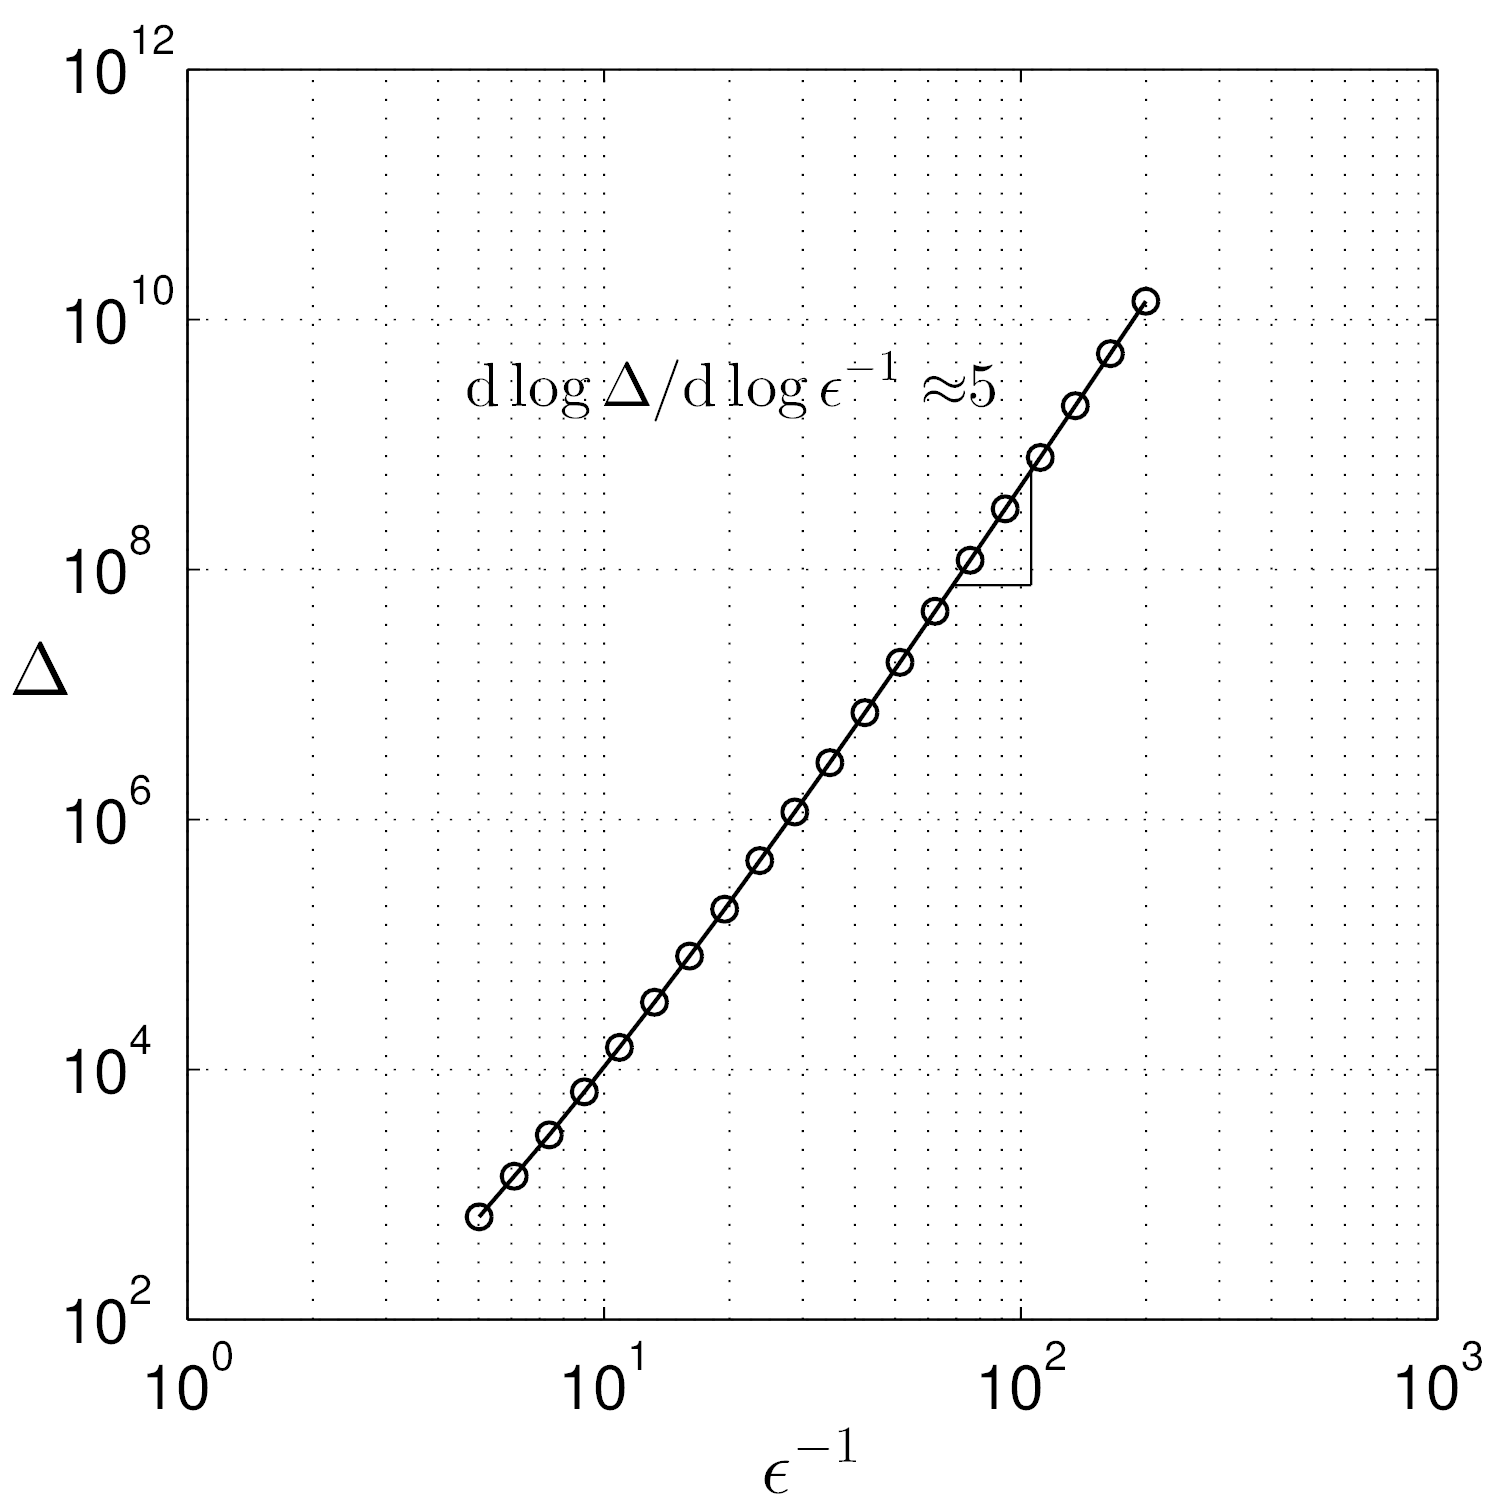
\includegraphics[scale=0.15]{pics/sup_fig6a.png}
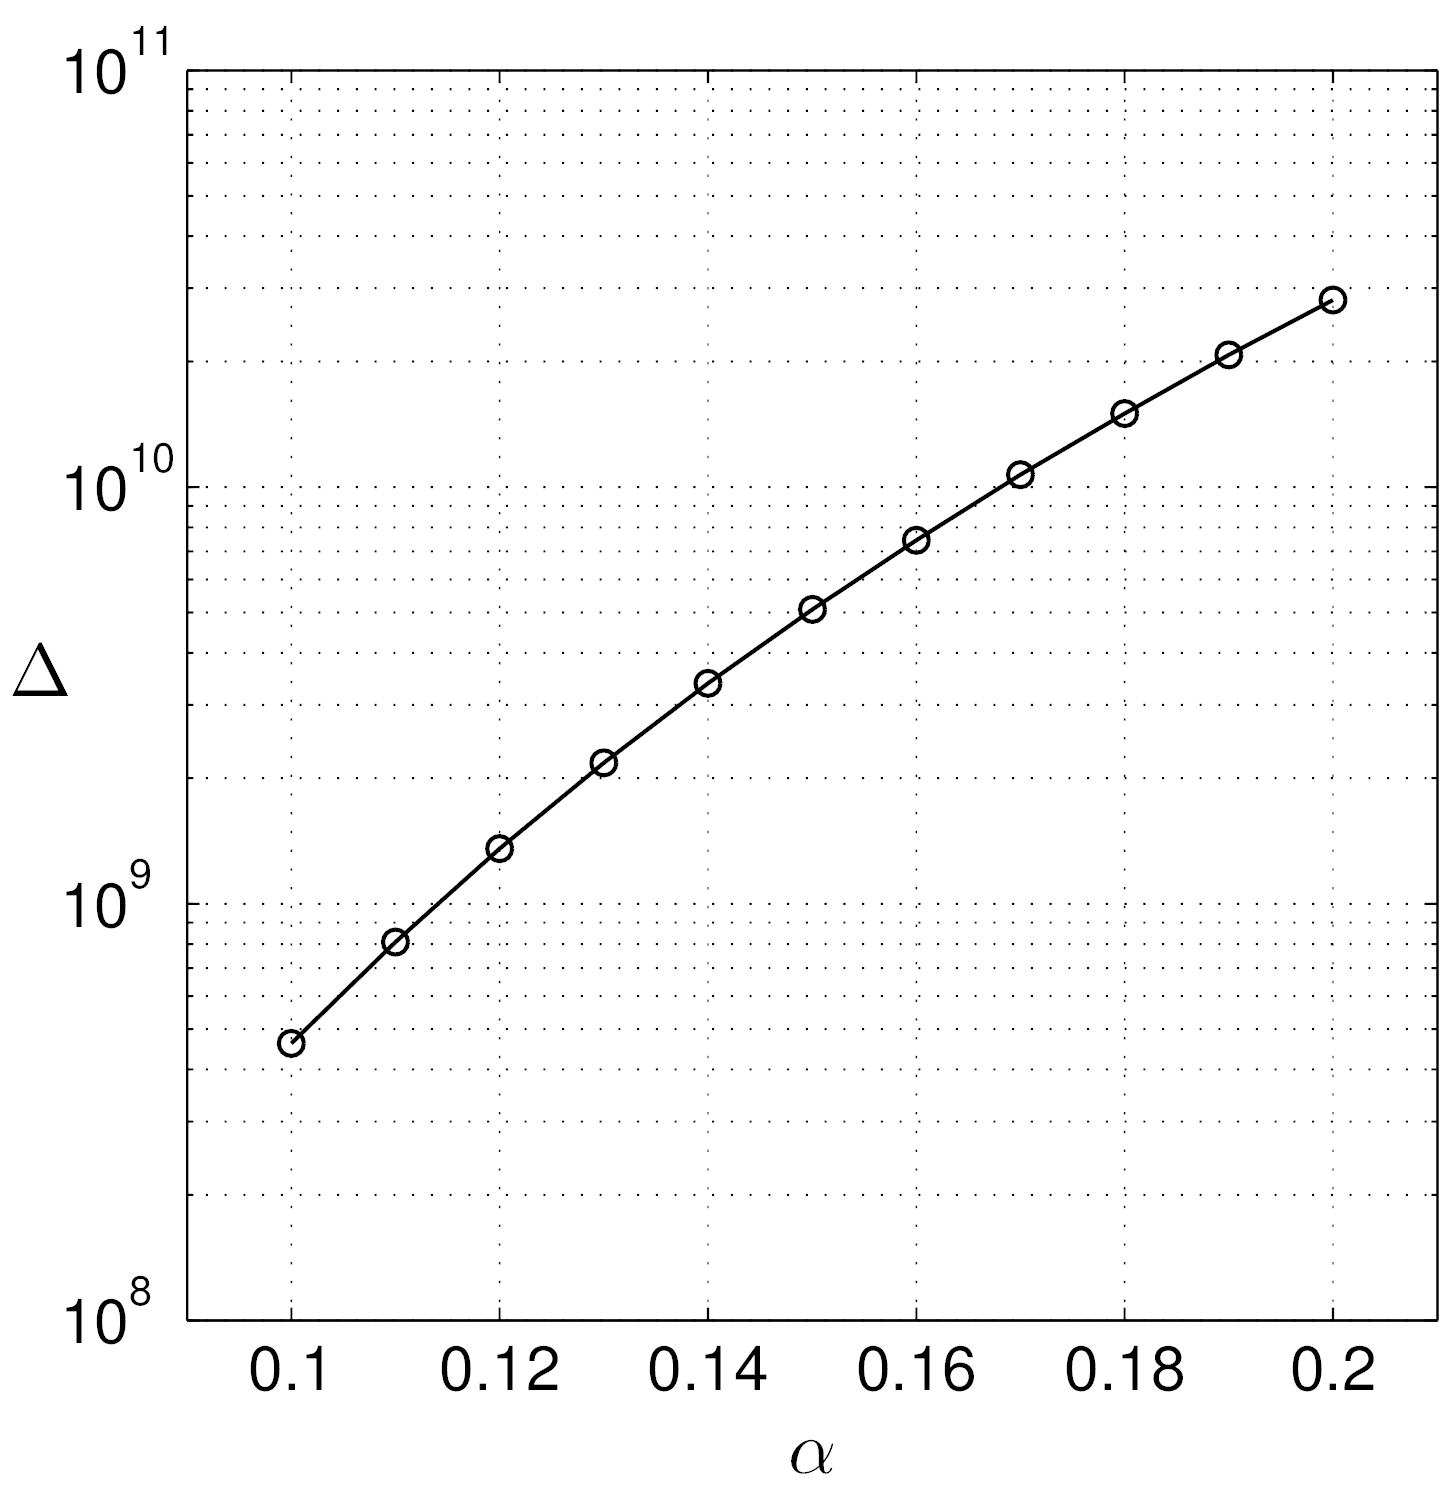
\includegraphics[scale=0.15]{pics/sup_fig6b.png}
\makebox[0.8cm]{}(a)\makebox[8cm]{}(b)
\caption{\normalsize (a) The scaling of minimum $\Delta$ needed to ensure $\|\Sigma_-(z)-H_\text{eff}\|\le\epsilon$ as a function of $\epsilon^{-1}$. Here we choose $\|H_\text{else}\|=0$, $\alpha=0.1$ and $\epsilon$ ranging from $10^{-0.7}$ to $10^{-2.3}$. The values of minimum $\Delta$ are numerically optimized \cite{footnote:num_op}. The slope of the line at large $\epsilon^{-1}$ is $4.97\approx{5}$, which provides evidence that with the assignments of ${\mu}=(\alpha\Delta^4/6)^{1/5}$, the optimal scaling of $\Delta$ is $\Theta(\epsilon^{-5})$. (b) The numerically optimized \cite{footnote:num_op} gap versus the desired coupling $\alpha$ in the target Hamiltonian. Here $\epsilon=0.01$ and $\|H_\text{else}\|=0$.}
\label{fig:ZZZ_fifth_Delta_eps}
\end{figure}

\refsec

\end{comment}

\newpage
\section{Direct Reduction}

Here we do not reduce $k$ by one order at a time (1B1 reduction) or by $\nicefrac{k}{2}$ at a time (SD reduction), but we directly reduce $k$-local terms to 2-local terms.
% Instead of reducing $k$ in a one-by-one (1B1) way, or in a $\nicefrac{k}{2}$-by-$\nicefrac{k}{2}$ way as in sub-division (SD) gadgets, we reduce from $k$-local to 2-local in one step, using $k$  auxiliary qubits for each $k$-local term.

\subsection{DR-JF (Jordan \& Farhi)}

\summarysec 

Express a sum of $k$-local terms as a sum of products of Pauli matrices $s_{ij}$, and define $k$ auxiliary qubits laelled by $a_{ij}$ for each term $i$, and make the transformmation:
 
\begin{equation}
\sum_i \alpha_i \prod_{j}^k s_{ij} \rightarrow \frac{-k(-\epsilon)^k}{(k-1)!} \sum_i \frac{1}{2}\left( k^2 - \sum_{jl}^k  z_{a_{ij}} z_{a_{il}} \right) + \epsilon \left( \alpha_i s_{i1}x_{i1} +  \sum_{j}^k s_{ij}x_{ij} \right) -f(\epsilon)\Pi,
\end{equation}

% there is some P_+ operator in JF's Eq. 14
% Above Eq. 8 of JF, tthere's an H_+ which we might need to care about. i.e project the whole of the baove equation onto one subspeace.

for some polynomial $f(\lambda)$. The result is a 2-local Hamiltonian with the same low-lying spectrum to within $\epsilon^{k+1}$ for sufficiently smmall $\epsilon$.  

\costsec
\begin{itemize}
\item Number of auxiliary qubits is $tk$ for $t$ terms. 
\item Unknown requirement for $\epsilon$.
\end{itemize}

\prossec
\begin{itemize}
\item All done in one step, so easier to implement than 1B1 and SD gadgets.
\end{itemize}

%
\conssec
\begin{itemize}
\item Requires 2 more auxiliary qubits per term than 1B1-KKR.
\item Unknown polynomial $f(\lambda)$
\end{itemize}

\examplesec

\refsec
\begin{itemize}
\item Original paper \cite{Jordan2008}.
\end{itemize}

\newpage
\section{Non-perturbative embeddings}

\subsection{NP-SJ (Subasi \& Jarzynski, 2016)}

\summarysec
Kato 1949.

\costsec

%\prossec
%\begin{itemize}
%\item
%\item
%\end{itemize}
%
%\conssec
%\begin{itemize}
%\item
%\item
%\end{itemize}

\examplesec

\refsec
\begin{itemize}
\item Original paper: \cite{Subas2016}.
\end{itemize}


\newpage
\part{{\normalsize {\underline{Appendix}}}}

%\section{Notation}
%
%The left Kronecker product by a $2\times2$ identity matrix is implied by Eqs. \eqref{eq:XZ+Z} and \eqref{eq:XX+Z} in the following way for qubit operators $q\in\{z,x\}$, assuming $i<j$:
%Subasi \& Jarzynski (2016)
%
%\begin{align}
%q_{i} & =\mathbf{1}^{\otimes i-1}q\mathbf{1}^{\otimes(N-i+1)}\\
%q_{i}\bar{q}_{j} & =\mathbf{1}^{\otimes i-1}q\mathbf{1}^{\otimes(j-1+i)}\bar{q}\mathbf{1}^{\otimes(N-j+1)}.
%\end{align}
%Thinking in this way, with this notation might take some time to get
%used to, but tens of thousands of people are comfortable thinking
%this way (including any undergraduate student after a 1-semester quantum
%computing course). You can now see that $H$ is a $2^{N}\times2^{N}$
%matrix with elements that are complex numbers. ``Minimizing the Hamiltonian''
%just means finding the eigenvector of this matrix with lowest eigenvalue.
%On a classical computer, the cost of finding this eigenvector is the
%cost of diagonalizing the matrix: $\mathcal{O}(2^{3N})$, but undergraduate
%level quantum mechanics tells us that any physical system's state
%(wavefunction, $\psi_{n}$) is an eigenvector of a Hamiltonian and
%the eigenvalue $E_{n}$ is just the energy associated with being in
%the $n^{{\rm th}}$ energy level: 
%\begin{equation}
%H\psi_{n}=E_{n}\psi_{n}.\label{eq:TISE}
%\end{equation}
%Eq. \ref{eq:TISE} is just the time-independent version of the Schroedinger
%equation, which you have at least heard of. The diagonal elements
%are the energies of the $n$ levels and the off-diagonals are associated
%with the propensity for tunnelling from level $n$ to level $m$.
%Any $2^{N}$ level system can be represented by $N$ spin-$\nicefrac{1}{2}$
%particles (\textbf{\uline{qubtis}}), and an example of a spin-$\nicefrac{1}{2}$
%particle is simply an electron. Some of the $N$ electrons will have
%spin up and some will have spin down, hence $2^{N}$ possibilities.
%So instead of $\mathcal{O}(2^{3N})$ operations on a classical computer
%for finding the eigenvector with lowest eigenvalue (and hence doing
%the completely arbitrary computation), we can just (for example) put
%$N$ electrons together %
%\begin{comment}
%such that the $2^{N}$ energy levels have energies $H_{ii}$ and tunelling
%amplitudes $H_{ij}$
%\end{comment}
%with the appropriate $H$ describing their energy, and then cool the
%system down to its ground state. This ground state is one out of $2^{N}$
%possible states , and the configuration of spin up and spin down electrons
%encodes the desired computation.
%
%\newpage
\section{Further Examples}

\examplesec \label{subsec:Example_Ramsey_deduc_reduc}
Here we show how deductions can arise naturally from the Ramsey number problem.
Consider $\mathbb{\mathcal{R}}(4,3)$ with $N=4$ nodes.
Consider a Hamiltonian:
\begin{equation}
H = (1-z_{12})(1-z_{13})(1-z_{23})+\ldots+(1-z_{23})(1-z_{24})(1-z_{34})+ z_{12}z_{13}z_{14}z_{23}z_{24}z_{34}.
\end{equation}

\begin{comment}
We should assume there are no 3-independent sets, so we have deductions:
$(1-z_{ij})(1-z_{ik})(1-z_{jk})=0$, for each $i,j,k$. 
\end{comment}
See \cite{Okada2015} for full details of how we arrive at this Hamiltonian.

Since we are assuming we have no 3-independent sets, we know that
$(1-z_{12})(1-z_{13})(1-z_{23})=0$, so $z_{12}z_{13}z_{23}=z_{12}z_{13}+z_{12}z_{23}+z_{13}z_{23}-z_{12}-z_{13}-z_{23}+1$.
This will be our deduction.

Using deduc-reduc we can substitute this into our 6-local term to get:
\begin{eqnarray}
H & = & 2(1-z_{12})(1-z_{13})(1-z_{23})+\ldots+(1-z_{23})(1-z_{24})(1-z_{34})+\\
 &  & z_{14}z_{24}z_{34}(z_{12}z_{13}+z_{12}z_{23}+z_{13}z_{23}-z_{12}-z_{13}-z_{23}+1).
\end{eqnarray}

We could repeat this process to remove all 5- and 4-local terms without adding any auxiliary qubits.
Note in this case the error terms added by deduc-reduc already appear in our Hamiltonian.

\section*{Acknowledgments}

\newpage
\bibliographystyle{apsrev4-1}
\bibliography{k-local-quadratization}

\end{document}
